%%%%%%%%%%%%%%%%%%%%%%%%%%%%%%%%%%%%%%%%%%%%%%%%%%%%%%%%%%%%%%%%%%%%%%%%%%%%%%%%
%%
%% Uppsala Beamer theme example by Frédéric Haziza <daz@it.uu.se>
%%
%% Describing beamerthemeUppsala version 2008/05/15
%%
%% If you have more than three sections or more than three subsections in at least
%% one section, you might want to use the [hideallsubsections] or
%% [hideothersubsections] switch.  In this case, only the current (sub-) section is
%% displayed in the sidebar and not the full overview.
%%
%% Options are:
%% ===========
%% * hideallsubsections, hideothersubsections
%% * nonumbers,totalnumber
%% * withnav, mylogo
%% * grey
%% * noprogressbar
%%
%% For the sidebar layout:
%% * subsectionsattop, sectionpathattop
%% 
%% Removed
%% =======
%% * sidebarshades
%%
%% Tip
%% ===
%% latex this file to see the theme in action
%%
%%%%%%%%%%%%%%%%%%%%%%%%%%%%%%%%%%%%%%%%%%%%%%%%%%%%%%%%%%%%%%%%%%%%%%%%%%%%%%%%

\documentclass{beamer}
%\documentclass[handout]{beamer}
%\documentclass[notes]{beamer}
%\documentclass[trans]{beamer}

\usetheme[hideothersubsections]{Uppsala}

\usepackage{hyperref}
\usepackage{pgf}
\usepackage{tikz}
\usepgflibrary{arrows}
\usepgflibrary{shapes}
\usetikzlibrary{%
  arrows,%
  calc,%
  fit,%
  patterns,%
  plotmarks,%
  shapes.geometric,%
  shapes.misc,%
  shapes.symbols,%
  shapes.arrows,%
  shapes.callouts,%
  shapes.multipart,%
  shapes.gates.logic.US,%
  shapes.gates.logic.IEC,%
  er,%
  automata,%
  backgrounds,%
  chains,%
  topaths,%
  trees,%
  petri,%
  mindmap,%
  matrix,%
  calendar,%
  folding,%
  fadings,%
  through,%
  positioning,%
  scopes,%
  decorations.fractals,%
  decorations.shapes,%
  decorations.text,%
  decorations.pathmorphing,%
  decorations.pathreplacing,%
  decorations.footprints,%
  decorations.markings,%
  shadows}

\usepackage{pgfplots}
\usepackage{pgfplotstable}
%\pgfplotsset{plot coordinates/math parser=false}
\usetikzlibrary{calc}
\pgfplotsset{compat=newest}
%\usetikzlibrary{colorbrewer}
 \usetikzlibrary{
   pgfplots.colorbrewer,
 }
\pgfplotsset{compat=newest}

%\usepackage[english]{babel} % or whatever
\usepackage[utf8]{inputenc} % or whatever

\usepackage{mathptmx}
\usepackage{helvet}
%\usepackage{courier}

\usepackage[T1]{fontenc}
% Or whatever. Note that the encoding and the font should match. If T1
% does not look nice, try deleting the line with the fontenc.

\usepackage[makeroom]{cancel}
\usepackage{cwpuzzle}
\usepackage[normalem]{ulem}
\usepackage{multirow,bigdelim}
\usepackage{pgfplots}
\usepackage{pgfplotstable}
\defbeamertemplate{description item}{align left}{\insertdescriptionitem\hfill}
\usepackage{colortbl}
\usepackage{wrapfig}

\usepackage[style=ieee,backend=bibtex]{biblatex}
\addbibresource{astra.bib}
\addbibresource{mybib.bib}
%\bibliography{astra}

%\bibliographystyle{abbrv}
\usepackage{astra}

\newcommand{\Dom}[1]{\text{dom}({#1})}
\newcommand{\Table}{\Constraint{Table}}

% SparseBitSet
\newcommand{\Words}{\texttt{words}}
\newcommand{\Index}{\texttt{index}}
\newcommand{\Mask}{\texttt{mask}}
\newcommand{\Limit}{\texttt{limit}}
\newcommand{\SparseBitSet}{\texttt{SparseBitSet}}
\newcommand{\Offset}{\localvar{offset}}

% CT Propagator
\newcommand{\Scp}{\texttt{vars}}
\newcommand{\CurrTable}{\texttt{validTuples}}
\newcommand{\Sval}{\texttt{S^{val}}}
\newcommand{\Ssup}{\texttt{S^{sup}}}
\newcommand{\LastSizes}{\texttt{lastSize}}
\newcommand{\Supports}{\texttt{supports}}
\newcommand{\Residues}{\texttt{residues}}

% Pseduo code
\newcommand{\ForEach}[1]{\textbf{foreach } {#1} \textbf{ do }}
\newcommand{\ForEachTo}[3]{\textbf{foreach } {#1} \textbf{ from } {#2} 
  \textbf{ to } {#3} \textbf{ do }}
\newcommand{\ForEachDownTo}[3]{\textbf{foreach } {#1} \textbf{ from } {#2} 
  \textbf{ downto } {#3} \textbf{ do }}
\newcommand{\Break}{\textbf{break~}}
\newcommand{\While}[1]{\textbf{while~} {#1} \textbf{~do~}}

\renewcommand{\algorithmicfor}{\textbf{Method}}
\renewcommand{\algorithmicdo}{}
\renewcommand{\algorithmicforall}{\textbf{foreach}}
%\renewcommand{\algorithmicwhile}{\textbf{foreach}}

\newcommand{\Func}[2]{\FOR{#1(#2)}}
\newcommand{\FuncRet}[3]{\FOR{#1(#2) \ : \ \textbf{#3}}}
\newcommand{\Endfunc}{\ENDFOR}
\newcommand{\To}{~\bf{to}~}
\newcommand{\Downto}{~{\bf{downto}}~}
\newcommand{\For}[3]{\FOR{${#1} \leftarrow {#2} \To {#3}$ \textbf{do}}}
\newcommand{\ForDown}[3]{\FOR{${#1} \leftarrow {#2} \Downto {#3}$ \textbf{do}}}
\newcommand{\FOREACH}[1]{\FORALL{{#1} \textbf{do}}}
\newcommand{\ENDFOREACH}{\ENDFOR}

\renewcommand{\algorithmiccomment}[1]{\hfill // #1}
\def\PROCEDURE{\item[\textbf{PROCEDURE}]}
\def\FAILED{\textbf{FAILED}}
\def\NOFIX{\textbf{NOFIX}}
\def\FIX{\textbf{FIX}}
\def\SUBSUMED{\textbf{SUBSUMED}}
\def\FAIL{\textbf{FAIL}}
\def\bool{\mathit{bool}}
\def\StatusMessage{\mathit{StatusMessage}}
\def\FindSupport{\textsc{FindSupport}}
\def\RemoveSupport{\textsc{RemoveSupport}}
\def\Extensional{\textsc{Extensional}}
\def\CompactTable{\textsc{CompactTable}}
\def\UpdateTable{\textsc{UpdateTable}}
\def\FilterDomains{\textsc{FilterDomains}}
\def\FixDomains{\textsc{FixDomains}}
\def\InitialiseCT{\textsc{InitialiseCT}}
\def\IndexOfFixed{\mathit{index\_of\_fixed}}


\newcommand{\ITE}[3]{\text{\bf ~if~} #1 \text{\bf ~then~} #2 \text{\bf ~else~} #3 \text{\bf ~endif}}

\newcommand{\function}[1]{\mathrm{#1}}
\newcommand{\localvar}[1]{\mathit{#1}}

\newlength\myindent
\setlength\myindent{2em}
\newcommand\bindent{%
  \begingroup
  \setlength{\itemindent}{\myindent}
  \addtolength{\algorithmicindent}{\myindent}
}
\newcommand\eindent{\endgroup}

\newcommand{\INDSTATE}[1][1]{\STATE\hspace{#1\algorithmicindent}}
\newcommand{\INDRETURN}[1][1]{\STATE\hspace{#1\algorithmicindent}\textbf{return~}}
\newcommand{\INDIF}[2][1]{\STATE\hspace{#1\algorithmicindent}
  \textbf{if~}{#2}\textbf{~then}}
\newcommand{\INDELSE}[1][1]{\STATE\hspace{#1\algorithmicindent}\textbf{else~}}
\newcommand{\INDELSEIF}[2][1]{\STATE\hspace{#1\algorithmicindent}
  \textbf{else if~}{#2}\textbf{~then}}

\newcommand{\CTpaper}[0]{DBLP:conf/cp/DemeulenaereHLP16}

\newcommand{\stressed}[1]{\emph{{\color{red!50}{#1}}}}

%% -----------------------------------------------------------
%% MISC. INFORMATION
%% -----------------------------------------------------------

\title{Implementation and Evaluation of a Compact-Table Propagator in Gecode}
%\subtitle{Bachelor's thesis}

\author[Linnea Ingmar | \emph{linnea.ingmar.3244@student.uu.se}] % appears in the footline
{Linnea Ingmar \\ <\texttt{linnea.ingmar.3244@student.uu.se}>}


\institute[Dept. of Information Technology] % appears in the footline
{
  The ASTRA Group\\ on Combinatorial Optimisation \\
  Uppsala University
}


\date[\today] % appears in the bottom of the sidebar
{\today}

%% \logo{...}

%% This is only inserted into the PDF information catalog. Can be left out.
\subject{Unofficial Beamer Theme for Uppsala University}

%% -----------------------------------------------------------
%% Extra ``local'' settings
%% -----------------------------------------------------------

% Comment out this, if you do not want the table of contents to pop up at
% the beginning of each (sub)section:
\AtBeginSection[]
{
  \begin{frame}<beamer> % with <beamer> => doesn't appear in handout mode
    \frametitle{Outline} %% Put the title you want, or none!
    %\tableofcontents[currentsection,currentsubsection]
    \tableofcontents[currentsection]
  \end{frame}
}

%% Unfolds piecewise element with shading.
%% Text appears, shaded, and the audience knows that somehting is coming
%% Note: if you set the number too high, the audience will try to read the 
%% text that now shows up more, and will be disturbed.
%% ``dynamic'' makes elements show gradually more and more.
\setbeamercovered{transparent=5}
%% \setbeamercovered{dynamic=5}

%% -----------------------------------------------------------

\begin{document}

\begin{frame}[plain] %% Gets the frame to fill up the page, no menu/sidebar/footline
  \titlepage
  
  \begin{figure}
    \begin{flushright}
        \begin{tabular}[t,right]{lr}
          Supervisor: & Mats Carlsson \\
          Reviewer:   & Pierre Flener
        \end{tabular}
      \end{flushright}
  \end{figure}

\end{frame}

\begin{frame}
    \frametitle{Outline}
    \tableofcontents[currentsection]
\end{frame}

\section{Background}

%\subsection{Constraint Programming}

\begin{frame}
  \frametitle{Kakuro puzzle}
  \begin{minipage}{0.45\textwidth}
    \includegraphics[scale=0.15]{kakuro.png}
  \end{minipage}
  \begin{minipage}{0.45\textwidth}
    \includegraphics[scale=0.15]{kakuro-sol.png}
  \end{minipage}

  \bigskip

  Assign the cells digits from~$1$ to~$9$ such that for each row and column:
  \begin{itemize}
    \item digits are distinct, and
    \item the sum of the digits is equal to the \emph{clue}
    \end{itemize}

\end{frame}

\begin{frame}
  \frametitle{Kakuro puzzle as a constraint problem (1)}
  \begin{minipage}{0.6\textwidth}
    \begin{description}
      \item[Variables] One per cell.
      \item[Domains] $\Set{1...9}$ for all variables.
      \item[Constraints] For each row and column: \stressed{distinct} digits,
        and the \stressed{sum} of the digits is equal to the clue.
    \end{description} 
  \end{minipage}
  \begin{minipage}{0.35\textwidth}
    \includegraphics[scale=0.15]{kakuro.png}
  \end{minipage}
\end{frame}

\begin{frame}
  \frametitle{Kakuro puzzle as a constraint problem (2)}
  \begin{minipage}{0.6\textwidth}
    \begin{description}
      \item[Variables] One per cell.
      \item[Domains] $\Set{1...9}$ for all variables.
      \item[Constraints] For each row and column: state the \stressed{possible
        combinations of values} that the variables can take.
    \end{description} 
  \end{minipage}
  \begin{minipage}{0.35\textwidth}
    \includegraphics[scale=0.15]{kakuro.png}
  \end{minipage}

  \bigskip
  \bigskip
  Row/column of size~$2$ and clue~$16$:~$\Tuple{7,9}$ and~$\Tuple{9,7}$
  are the only combinations.
\end{frame}

\begin{frame}
  \frametitle{\Table~constraints}
  \begin{definition}[\Table~constraint]
    A \Table~constraint lists the possible combinations of values
    that the variables can take as a sequence of~$n$-tuples.
  \end{definition}

  \bigskip
  \bigskip

  \begin{tabular}{lccr}
    %\Table($\Set{x_0,x_1}$, $[\Tuple{7,9},\Tuple{9,7}]$)\\
    \bigskip
    \begin{tabular}{cc}
      $x_0$ & $x_1$ \\
      \hline
      $7$   & $9$ \\
      $9$   & $7$ \\
    \end{tabular}
            &
            &
            &
              \phantom{foo}
              \includegraphics[scale=0.2]{kakuro-hint.png}
    
  \end{tabular}
\end{frame}



% - CSP
% \begin{frame}
%   \frametitle{Constraint problems (definition)}
%   \begin{definition}[Constraint problem]
%     A \textbf{constraint satisfaction problem (CSP)} is a 
%     triple\\
%     \begin{center}
%       $\left<V,D,C\right>$\\      
%     \end{center}
%     where: \\
%     \begin{itemize}
%       \item $V = v_1, \ldots, v_n$ is a finite sequence of variables,
%       \item $D = D_1, \ldots, D_n$ is a finite sequence of domains, that are
%         possible values for the respective variable,
%       \item $C = \Set{c_1, \ldots, c_m}$ is a finite set of constraints, 
%         each on a subset of~$V$. 
%         Express relations among the variables that have to be true.
%     \end{itemize}
%   \end{definition}
% \end{frame}

\begin{frame}
  \frametitle{Solving Constraint Problems}
  \begin{minipage}{0.6\textwidth}
    \begin{description}
    \item[Solution]
      A complete
      variable-value assignment satisfying the constraints.\\
      \smallskip
      (Sometimes: maximises/minimises given function.)
    \end{description}
  \end{minipage}
  \begin{minipage}{0.35\textwidth}
    \includegraphics[scale=0.15]{kakuro-sol.png} \\
  \end{minipage}
  
  \begin{minipage}{0.6\textwidth}
    \begin{itemize}
    \item Solutions are found by \textbf{search}
      \begin{itemize}
      \item \alt<2>{\textbf{Propagation}}{Propagation}
      \item \alt<2>{\color{gray}Branching}{Branching}
      \end{itemize}
    \end{itemize}
  \end{minipage}
  \begin{minipage}{0.15\textwidth}
    \includegraphics[scale=0.3]{searchtree.png}
  \end{minipage}
  % \begin{minipage}{0.15\textwidth}
  %   \tiny
  %   \begin{tabular}[t]{c}
  %     Propagation \\
  %     Branching \\
  %     Propagation \\
  %     Branching \\
  %   \end{tabular}
  % \end{minipage}
  
\end{frame}


% - Store

\begin{frame}
  \frametitle{Constraint Propagation}
  Important concepts:
  \begin{itemize}
    \item Constraint store
    \item Propagator
    %\item Constraint propagation
  \end{itemize}
\end{frame}

\begin{frame}
  \frametitle{Constraint Stores}
  \begin{definition}[Constraint store]
    A \textbf{constraint store}~$s$ is a function mapping variables
    to domains:
    \begin{center}
      $s: variables \mapsto domains$
    \end{center}
  \end{definition}

  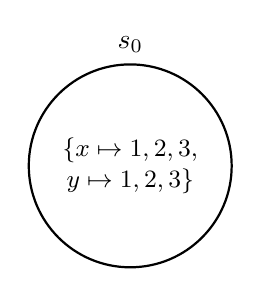
\begin{tikzpicture}[->,>=stealth',auto,node distance=3cm,
    thick,main node/.style={circle,draw,font=\sffamily\Large\bfseries}]
    \node[label={$s_0$},draw,circle](1){
      \small
      \begin{tabular}{c}
        $\{x \mapsto \Set{1,2,3},$\\ 
        $y\mapsto\Set{1,2,3}\}$
      \end{tabular}
    };
    
  \end{tikzpicture}

\end{frame}

\begin{frame}
  \frametitle{Propagators}
  \begin{definition}[Propagator]
    A \textbf{propagator}~$p$ is a function mapping stores to stores:
    \begin{center}
      $p: store \mapsto store$ 
    \end{center}
  \end{definition}

  \begin{itemize}
  \item   Implement constraints
  % \item   Prune values from the domains that are in conflict 
  %   with the constraint
  \end{itemize}

  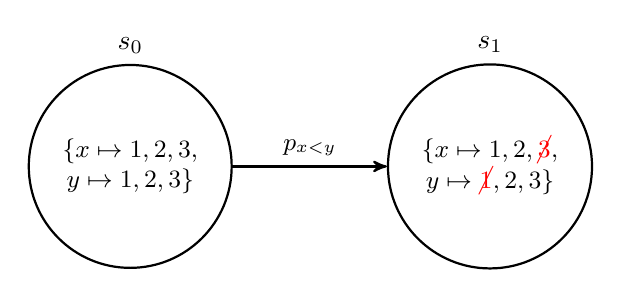
\begin{tikzpicture}[->,>=stealth',auto,node distance=3cm,
  thick,main node/.style={circle,draw,font=\sffamily\Large\bfseries}]
    \node[label=$s_0$,draw,circle](1){
      \small
      \begin{tabular}{c}
        $\{x \mapsto \Set{1,2,3},$\\ 
        $y\mapsto\Set{1,2,3}\}$
      \end{tabular}
    };
    \node[label=$s_1$,draw,circle,right of=1,node distance=13em](2){
      \small
      \begin{tabular}{c}
        $\{x \mapsto \Set{1,2,{\color{red}\cancel{3}}},$\\ 
        $y\mapsto\Set{{\color{red}\cancel{1}},2,3}\}$
      \end{tabular}
    };
    \path[every node/.style={font=\sffamily\small}] 
    (1) edge node [bend right] {$p_{x<y}$} (2);
    
  \end{tikzpicture}

\end{frame}

\begin{frame}
  \frametitle{Constraint Propagation}
  %Prune values from the variables that  
  \begin{minipage}{0.5\textwidth}
    \only<1>{$x_0 \in \Set{1,2,3,4,5,6,7,8,9}$}
    \only<2>{$x_0 \in \Set{\cancel{\color{blue}1},\cancel{\color{blue}2},\cancel{\color{blue}3},\cancel{\color{blue}4},\cancel{\color{blue}5},\cancel{\color{blue}6},7,\cancel{\color{blue}8},9}$}
    \only<3->{$x_0 \in \Set{\cancel{\color{blue}1},\cancel{\color{blue}2},\cancel{\color{blue}3},\cancel{\color{blue}4},\cancel{\color{blue}5},\cancel{\color{blue}6},\textbf{7},\cancel{\color{blue}8},\cancel{\color{purple}9}}$} \\
    \only<1>{$x_1 \in \Set{1,2,3,4,5,6,7,8,9}$}
    \only<2-3>{$x_1 \in \Set{\cancel{\color{blue}1},\cancel{\color{blue}2},\cancel{\color{blue}3},\cancel{\color{blue}4},\cancel{\color{blue}5},\cancel{\color{blue}6},7,\cancel{\color{blue}8},9}$}
    \only<4->{$x_1 \in \Set{\cancel{\color{blue}1},\cancel{\color{blue}2},\cancel{\color{blue}3},\cancel{\color{blue}4},\cancel{\color{blue}5},\cancel{\color{blue}6},\cancel{\color{blue}7},\cancel{\color{blue}8},\textbf{9}}$}\\
    $\ldots$ \\
    \only<1-2>{$x_4 \in \Set{1,2,3,4,5,6,7,8,9}$}
    \only<3->{$x_4 \in \Set{\cancel{\color{purple}1},\textbf{2},\cancel{\color{purple}3},\cancel{\color{purple}4},\cancel{\color{purple}5},\cancel{\color{purple}6},\cancel{\color{purple}7},\cancel{\color{purple}8},\cancel{\color{purple}9}}$}\\
    $\ldots$
    %$\Table(\Set{x_0,x_1},\Set{\Tuple{7,9},\Tuple{9,7}})$
    
    \begin{tabular}{ccc}
      
      \begin{tabular}{!{\color{blue}\vrule}cc!{\color{blue}\vrule}}
        \arrayrulecolor{blue}\hline
        $x_0$ & $x_1$ \\
        \hline
        $7$   & $9$ \\
        \alt<4>{\sout{$9$}   & \sout{$7$}} 
                               {$9$   & $7$} \\
        \arrayrulecolor{blue}\hline
        
      \end{tabular} & 
                         \only<1>{
                          \begin{tabular}{!{\color{purple}\vrule}cc!{\color{purple}\vrule}}
                            \arrayrulecolor{purple}\hline
                            $x_0$ & $x_4$ \\
                            \hline
                            $1$   & $8$ \\
                            $2$   & $7$ \\
                            $3$   & $6$ \\
                            $4$   & $5$ \\
                            $5$   & $4$ \\
                            $6$   & $3$ \\
                            $7$   & $2$ \\
                            $8$   & $1$ \\
                            \arrayrulecolor{purple}\hline
                          \end{tabular} & $\ldots$}
                          \only<2->{
                          \begin{tabular}{!{\color{purple}\vrule}cc!{\color{purple}\vrule}}
                            \arrayrulecolor{purple}\hline
                            $x_0$ & $x_4$ \\
                            \hline
                            \sout{$1$}   & \sout{$8$} \\
                            \sout{$2$}   & \sout{$7$} \\
                            \sout{$3$}   & \sout{$6$} \\
                            \sout{$4$}   & \sout{$5$} \\
                            \sout{$5$}   & \sout{$4$} \\
                            \sout{$6$}   & \sout{$3$} \\
                            $7$   & $2$ \\
                            \sout{$8$}  &  \sout{$1$}\\
                            \arrayrulecolor{purple}\hline
                          \end{tabular} & $\ldots$}

    \end{tabular}

  \end{minipage}
  \begin{minipage}{0.45\textwidth}
    \alt<4>
    {\includegraphics[scale=0.2]{kakuro-vars-color-ass.png}}
    {\includegraphics[scale=0.2]{kakuro-vars-color.png}}

  \end{minipage}
\end{frame}

%\subsection{Gecode}

\begin{frame}

 
  \frametitle{Gecode}
  \textbf{Gecode} (Generic Constraint Development Environment)

  \begin{itemize}
    \item A constraint programming solver (a software that solves constraint problems).
    \item Written in C++, modular, extensible, and has state-of-the-art performance.
    \item Supports the programming of new propagators.
    \item Uses copying during branching, not trailing
    \item   Two existing propagators for the~\Table~constraint
  \end{itemize}

  % , and one for the 
  % related constraint~\Constraint{Regular}.
  
    \begin{figure}[t]
    \begin{center}
      \includegraphics[scale=0.25]{gecode.png}
    \end{center}
  \end{figure}


\end{frame}

%\subsection{The Compact-Table algorithm}

\begin{frame}
  \frametitle{Compact Table}
  \includegraphics[scale=0.45]{compact-table.png}
\end{frame}

\begin{frame}
  \frametitle{Compact-Table}
  % Efficient
  \begin{itemize}
  \item   A new propagation algorithm for the~\Table~constraint
  \item   First implemented in OR-tools (uses trailing during branching)
  \item   Published in a 2016 paper~\cite{\CTpaper} -- the starting
    point of this project
  \item   Promising results -- outperforms previously known algorithms in the
    benchmarks in \cite{\CTpaper}
  \item   Previously no attempt to implement it in Gecode 
    (to the best of my knowledge)
  \end{itemize}

\end{frame}

\section{The Compact-Table Algorithm}

% \begin{frame}
%   \frametitle{Fields}
%   \begin{description}
%     \item[\CurrTable] \emph{Sparse bit-set:} Stores indices of valid tuples
%     \item[\Supports]  \emph{Array of bit-sets:} \Supports[$x,a$] stores which tuples
%       are supports for the variable-value pair~$\Tuple{x,a}$
%     \item[\Residues]  \emph{Array of ints:} $\Residues[x,a]$ is the index in \CurrTable~where
%       a support for~$\Tuple{x,a}$ was found the last time it was sought for
%   \end{description}
%   \bigskip
%   % Where:
%   % \emph{Valid tuple~:} All values in~$\tau$ are in the domains of the variables
%   % \emph{Support:} $\tau$ is a support for  

% \end{frame}

% \begin{frame}
%   \frametitle{The Compact-Table Algorithm}
%   \begin{itemize}
%   \item \textbf{Initialisation}
%   \item \color{gray}Variable modifications
%   \item Filtering
%    \item {\color{gray}Putting it all together}
%   \end{itemize}
% \end{frame}

\begin{frame}
%  \frametitle{The Compact-Table Algorithm}
  \frametitle{Initialisation}
  \small
  \only<1-5>{
    $\Dom{x_0} = \Dom{x_1} = \Dom{x_2} = \Set{1,2,3,4}$
  }
  \only<6->{
    $\Dom{x_0} = \Set{1,2,{\color{red}\cancel{3}},4}$\\
    $\Dom{x_1} = \Dom{x_2} = \Set{1,2,3,4}$
  }

  \bigskip

  \begin{tabular}{l}

    \only<4->{
    %\CurrTable: bit-set with valid tuples\\
    %\phantom{foo}\\
    \small
    \begin{tabular}{cc}
      %\phantom{\texttt{words}}
      \phantom{$\Tuple{x_0,2}$}
      &
        \begin{tabular}{|cccccccc|c}
          \cline{1-8}
          {\textbf{1}} & {\textbf{1}} & {\textbf{1}} & {\textbf{1}} & {\textbf{1}}& {\textbf{1}}& {\textbf{1}} & {\textbf{1}} & \rdelim\}{1}{3mm}[\CurrTable] \\
          \cline{1-8}
        \end{tabular}
    \end{tabular}

    \bigskip
    }
    \\
    \only<5->{
    %\Supports: \\
    %\phantom{foo}\\
    \begin{tabular}{ccc}
      $\Tuple{x_0,1}$
      & 
        \begin{tabular}{|cccccccc|}
          \hline
          0 & \textbf{1} & 0 & 0 & \textbf{1} & 0 & 0 & 0 \\
        \end{tabular}
      &
        \rdelim\}{5}{3mm}[\texttt{supports}]
      \\
      $\Tuple{x_0,2}$
      & 
        \begin{tabular}{|cccccccc|}
          \textbf{1} & 0 & \textbf{1} & 0 & 0 & \textbf{1} & \textbf{1} & 0 \\
        \end{tabular}
      \\
      $\Tuple{x_0,3}$
      & 
        \begin{tabular}{|cccccccc|}
          \alt<6->{{\color{red}0} & \color{red}0 & \color{red}0 & \color{red}0 & \color{red}0 & \color{red}0 & \color{red}0 & {\color{red}0}} 
              {0 & 0 & 0 & 0 & 0 & 0 & 0 & 0} \\
          
        \end{tabular}
      \\
      $\ldots$
      \\
      $\Tuple{x_2,4}$
      & 
        \begin{tabular}{|cccccccc|}
          \textbf{1} & 0 & 0 & 0 & 0 & 0 & 0 & 0 \\
          \hline
        \end{tabular}
      \\
    \end{tabular}
        
    \bigskip
    } 
    \\
    \only<1>{
    \small
        \begin{tabular}{|c|cccccccccccccccc|}
          \hline
          $x_0$ & 1 & 2 & 1 & 2 & 6 & 7 & 4 & 1 & 7 & 8 & 2 & 0 & 2 & 5 & 4 \\
          $x_1$ & 5 & 1& 3 & 4 & 5 & 7 & 2 & 1 & 8 & 9 & 2 & 0 & 3 & 8 & 3 \\
          $x_2$ & 8 & 4& 2 & 2 & 9 & 8 & 1 & 1 & 9 & 6 & 3 & 0 & 1 & 5 & 1 \\
          \hline
        \end{tabular}}
    \only<2>{
    \small
    \begin{tabular}{|c|ccccccccccccccc|}
      \hline
      $x_0$ & 1 & \textbf{2} & \textbf{1} & \textbf{2} & 6 & 7 & \textbf{4} & \textbf{1} & 7 & 8 & \textbf{2} & 0 & \textbf{2} & 5 & \textbf{4} \\
      $x_1$ & 5 & \textbf{1}& \textbf{3} & \textbf{4} & 5 & 7 & \textbf{2} & \textbf{1} & 8 & 9 & \textbf{2} & 0 & \textbf{3} & 8 & \textbf{3} \\
      $x_2$ & 8 & \textbf{4}& \textbf{2} & \textbf{2} & 9 & 8 & \textbf{1} & \textbf{1} & 9 & 6 & \textbf{3} & 0 & \textbf{1} & 5 & \textbf{1} \\
      \hline
    \end{tabular}
    }
    
    \small
    \begin{tabular}{cc}
      &
        \only<3->{
        \begin{tabular}{|c|cccccccc|}
          \hline
          $x_0$ & \textbf{2}& \textbf{1} & \textbf{2} & \textbf{4} & \textbf{1} & \textbf{2} & \textbf{2} & \textbf{4} \\
          $x_1$ & \textbf{1}& \textbf{3} & \textbf{4} & \textbf{2} & \textbf{1} & \textbf{2} & \textbf{3} & \textbf{3} \\
          $x_2$ & \textbf{4}& \textbf{2} & \textbf{2} & \textbf{1} & \textbf{1} & \textbf{3} & \textbf{1} & \textbf{1} \\
          \hline
          \multicolumn{1}{c}{} &
          \multicolumn{1}{c}{\tiny 0} &
          \multicolumn{1}{c}{\tiny 1}&
          \multicolumn{1}{c}{\tiny 2}&
          \multicolumn{1}{c}{\tiny 3}&
          \multicolumn{1}{c}{\tiny 4}&
          \multicolumn{1}{c}{\tiny 5}&
          \multicolumn{1}{c}{\tiny 6}&
          \multicolumn{1}{c}{\tiny 7}
        \end{tabular}
      }

    \end{tabular}

  \end{tabular}

\end{frame}


% \begin{frame}
%   \frametitle{The Compact-Table Algorithm}
%   \begin{itemize}
%   \item {\color{gray}Initialisation}
%   \item \textbf{Variable modifications}
%   \item {\color{gray}Filtering}
%   \item {\color{gray}Putting it all together}
%   \end{itemize}
% \end{frame}
\begin{frame}
  \frametitle{Variable Modifications}
  When a variable~$x$ is modified, there are two ways to update~\CurrTable:
  \smallskip
  \begin{description}
    \item[$\Cardinality{\Delta_x} < \Cardinality{\Dom{x}}$] Incremental update
    \item[$\Cardinality{\Delta_x} \geq \Cardinality{\Dom{x}}$] Reset-based update
  \end{description}

  \bigskip
  \bigskip

  \begin{tabular}{|c|}
    \hline
    $\Delta_x$: set of removed values \\
    \hline
  \end{tabular}

\end{frame}

\begin{frame}
  %\frametitle{The Compact-Table Algorithm}
  \frametitle{Variable Modifications}
  \framesubtitle{Reset-based update}

  \only<2->{
    \begin{tabular}{c}
      \small
      \begin{tabular}{ccc}
        \texttt{words} 
        & 
          \begin{tabular}{|cccccccc|}
            \hline
            \alt<7->{{\color{red}0} & {\textbf{1}} & {\textbf{1}} & {\color{red}0} & {\color{red}0}& {\color{red}0}& {\textbf{1}} & {\textbf{1}}}
            {{\textbf{1}} & {\textbf{1}} & {\textbf{1}} & {\textbf{1}} & {\textbf{1}}& {\textbf{1}}& {\textbf{1}} & {\textbf{1}}} \\
            \hline
          \end{tabular}
        &
          \rdelim\}{2}{1mm}[\tiny \CurrTable]
        \\
        \texttt{mask} 
        &
          \begin{tabular}{|cccccccc|}
            \hline
            \alt<5->{{0} & {\textbf{1}} & {\textbf{1}} & {0} & {0}& {0}& {\textbf{1}} & {\textbf{1}}}
            {{0} & {0} & {0} & {0} & {0}& {0}& {0} & {0}} \\
            \hline
          \end{tabular} 
        \\
        \only<3->{
        \phantom{foo} \\
        $\Supports[x_1,3]$ 
        & 
          \begin{tabular}{|cccccccc|}
            \hline
            0 & \textbf{1} & 0 & 0 & 0 & 0 & \textbf{1} & \textbf{1} \\
            \hline
          \end{tabular}
        \\
        $\Supports[x_1,4]$
        & 
          \begin{tabular}{|cccccccc|}
            \hline
            0 & 0 & \textbf{1} & 0 & 0 & 0 & 0 & 0 \\
            \hline
          \end{tabular}
        \\
        }
        \only<8->{
        \phantom{foo} \\
        $x_0$
        &
          \small
          \begin{tabular}{|cccccccc|}
            \hline
            {\color{red}2}& \textbf{1} & \textbf{2} & {\color{red}4} & {\color{red}1} & {\color{red}2} & \textbf{2} & \textbf{4} \\
          \end{tabular}
        \\
        $x_1$
        &
          \small
          \begin{tabular}{|cccccccc|}
            {\color{red}1}& \textbf{3} & \textbf{4} & {\color{red}2} & {\color{red}1} & {\color{red}2} & \textbf{3} & \textbf{3} \\
          \end{tabular}
        \\
        $x_2$
        &
        \small
          \begin{tabular}{|cccccccc|}
            {\color{red}4}& \textbf{2} & \textbf{2} & {\color{red}1} & {\color{red}1} & {\color{red}3} & \textbf{1} & \textbf{1} \\
            \hline
          \end{tabular}
        \\
        }
      \end{tabular}
      \\
      \only<4>{
      \phantom{foo}\\
      \texttt{mask} = \Supports[$x_1,3$] | \Supports[$x_1,4$]\\
      }
      \only<6>{
        \phantom{foo}\\
      \small
      \texttt{words} = \texttt{words} \& \texttt{mask} \\
      }
    \end{tabular}
    \\
  }
  
  \bigskip

  $\Dom{x_0} = \Set{1,2,4}$\\
  $\Dom{x_1} = \Set{\cancel{1},\cancel{2},3,4}$\\
  $\Dom{x_2} = \Set{1,2,3,4}$

\end{frame}

\begin{frame}
  %\frametitle{The Compact-Table Algorithm}
  \frametitle{Variable Modifications}
  \framesubtitle{Incremental update}

  \only<2->{
    \begin{tabular}{c}
      \small
      \begin{tabular}{ccc}
        \texttt{words} 
        & 
          \begin{tabular}{|cccccccc|}
            \hline
            \alt<7->{{\color{red}0} & {\textbf{1}} & {\textbf{1}} & {\color{red}0} & {\color{red}0}& {\color{red}0}& {\textbf{1}} & {\textbf{1}}}
            {{\textbf{1}} & {\textbf{1}} & {\textbf{1}} & {\textbf{1}} & {\textbf{1}}& {\textbf{1}}& {\textbf{1}} & {\textbf{1}}} \\
            \hline
          \end{tabular}
        &
          \rdelim\}{2}{1mm}[\tiny \CurrTable]
        \\
        \texttt{mask} 
        &
          \begin{tabular}{|cccccccc|}
            \hline
            \alt<5->{\textbf{1} & 0 & 0 & \textbf{1} & \textbf{1} & \textbf{1} & 0 & 0}
            {{0} & {0} & {0} & {0} & {0}& {0}& {0} & {0}} \\
            \hline
          \end{tabular} 
        \\
        \only<3->{
        \phantom{foo} \\
        $\Supports[x_1,1]$ 
        & 
          \begin{tabular}{|cccccccc|}
            \hline
            \textbf{1} & 0 & 0 & 0 & \textbf{1} & 0 & {0} & {0} \\
            \hline
          \end{tabular}
        \\
        $\Supports[x_1,2]$
        & 
          \begin{tabular}{|cccccccc|}
            \hline
            0 & 0 & {0} & \textbf{1} & 0 & \textbf{1} & 0 & 0 \\
            \hline
          \end{tabular}
        \\
        }
        \only<8->{
        \phantom{foo} \\
        $x_0$
        &
          \small
          \begin{tabular}{|cccccccc|}
            \hline
            {\color{red}2}& \textbf{1} & \textbf{2} & {\color{red}4} & {\color{red}1} & {\color{red}2} & \textbf{2} & \textbf{4} \\
          \end{tabular}
        \\
        $x_1$
        &
          \small
          \begin{tabular}{|cccccccc|}
            {\color{red}1}& \textbf{3} & \textbf{4} & {\color{red}2} & {\color{red}1} & {\color{red}2} & \textbf{3} & \textbf{3} \\
          \end{tabular}
        \\
        $x_2$
        &
        \small
          \begin{tabular}{|cccccccc|}
            {\color{red}4}& \textbf{2} & \textbf{2} & {\color{red}1} & {\color{red}1} & {\color{red}3} & \textbf{1} & \textbf{1} \\
            \hline
          \end{tabular}
        \\
        }
      \end{tabular}
      \\
      \only<4>{
      \phantom{foo}\\
      \texttt{mask} = \Supports[$x_1,1$] | \Supports[$x_1,2$]\\
      }
      \only<6>{
        \phantom{foo}\\
      \small
      \texttt{words} = \texttt{words} \& !\texttt{mask} \\
      }
    \end{tabular}
    \\
  }
  
  \bigskip

  $\Dom{x_0} = \Set{1,2,4}$\\
  $\Dom{x_1} = \Set{\cancel{1},\cancel{2},3,4}$\\
  $\Dom{x_2} = \Set{1,2,3,4}$

\end{frame}


\begin{frame}
  %\frametitle{Compact-Table Algorithm}
  \frametitle{Filtering}
    
  \begin{itemize}
    \item Intersect every support entry with~$\CurrTable$
    \item Remove value if intersection is empty
  \end{itemize}
  
  \bigskip

  \begin{tabular}{c}
      \CurrTable:\\
      \small
      \begin{tabular}{cc}
        \texttt{words} 
        & 
          \begin{tabular}{|cccccccc|}
            \hline
            {0} & {\textbf{1}} & {\textbf{1}} & {0} & {0} & {0} & {\textbf{1}} & {\textbf{1}} \\
            \hline
          \end{tabular}
      \end{tabular} \\
    \\
    \& \\
    \phantom{foo}
    \\
    \small
    \begin{tabular}{cc}
      $\Tuple{x_2,1}$
        & 
          \begin{tabular}{|cccccccc|}
            \hline
            \alt<2->{\color{green}0 & \color{green}0 & \color{green}0 & \color{green}\textbf{1} & \color{green}\textbf{1} & \color{green}0 & \color{green}\textbf{1} & \color{green}\textbf{1}}
            {0 & 0 & 0 & \textbf{1} & \textbf{1} & 0 & \textbf{1} & \textbf{1}} \\
          \end{tabular}
        \\
        $\Tuple{x_2,2}$
        & 
          \begin{tabular}{|cccccccc|}
            \alt<3->
            {\color{green}0 & \color{green}\textbf{1} & \color{green}\textbf{1} & \color{green}0 & \color{green}0 & \color{green}0 & \color{green}0 & \color{green}0}
            {0 & \textbf{1} & \textbf{1} & 0 & 0 & 0 & 0 & 0} \\
          \end{tabular}
        \\
        $\Tuple{x_2,3}$
        & 
          \begin{tabular}{|cccccccc|}
            \alt<4->
            {\color{red}0 & \color{red}0 & \color{red}0 & \color{red}0 & \color{red}0 & \color{red}\textbf{1} & \color{red}0 & \color{red}0}
            {0 & 0 & 0 & 0 & 0 & \textbf{1} & 0 & 0} \\
          \end{tabular}
        \\
        $\Tuple{x_2,4}$
        & 
          \begin{tabular}{|cccccccc|}
            \alt<5->
            {\color{red}\textbf{1} & \color{red}0 & \color{red}0 & \color{red}0 & \color{red}0 & \color{red}0 & \color{red}0 & \color{red}0} 
            {\textbf{1} & 0 & 0 & 0 & 0 & 0 & 0 & 0} \\
            \hline
          \end{tabular}
      \\
      \end{tabular}
    \\
    \phantom{foo} \\
    \alt<6>    
    {$\Dom{x_2} = \Set{1,2,{\color{red}\cancel{3}},{\color{red}\cancel{4}}}$}
    {$\Dom{x_2} = \Set{1,2,3,4}$}
    \end{tabular}
    
\end{frame}

\begin{frame}
  \frametitle{Sparse bit-set}
  \begin{itemize}
    \item Bit-wise operations are performed on non-zero words only
  \end{itemize}
  \bigskip
  \small
  \CurrTable:
  \begin{tabular}{|ccccc|}
    \hline
                   & \tiny 0 & \tiny 1 & \tiny 2& \tiny 3 \\
    \texttt{words} = & \textbf{0} \textbf{1} \textbf{0} \textbf{0} & \textbf{0} \textbf{0} \textbf{1} \textbf{0} & \alt<2>{\color{red}0 0 0 0}{\textbf{1} \textbf{0} \textbf{0} \textbf{0}} & \textbf{1} \textbf{0} \textbf{0} \textbf{1}\\
    \texttt{mask} = & 0 0 0 0 & 0 0 0 0 & 0 0 0 0 & 0 0 0 0 \\
    \texttt{index} = & \alt<2>{[\textbf{0}, \textbf{1}, {\color{red}\textbf{3}}, {\color{red}2}]}{[\textbf{0}, \textbf{1}, {\textbf{2}}, \textbf{3}]} &&& \\
    \texttt{limit} = & \alt<2>{\color{red}2}{3} & & & \\
    \hline
  \end{tabular}
\end{frame}


\section{Evaluation}
% \subsection{Setup}
% \subsection{Results}
% \subsection{Discussion}
%\subsection{Setup}

\begin{frame}
  \frametitle{Experiments}
  
  \begin{itemize}
    \item   Compared CT against
      \begin{itemize}
      \item $2$~existing propagators for \Table
      \item $1$~propagator for \Constraint{Regular}
      \end{itemize} 
    \item Same benchmark set that was used in~\cite{\CTpaper}
      (translated to MiniZinc)
      \begin{itemize}
        \item $1507$~instances over~$30$ series 
        \item Table sizes:~$1-1.6 \cdot 10^6$ tuples
        \item Arities:~$2-20$ variables
        \item Domain sizes:~$1-1000$
        \item Available at \url{https://bitbucket.org/pschaus/xp-table}
          ($15$ GB of uncompressed files)
      \end{itemize}
      
  \end{itemize}
\end{frame}

\begin{frame}
  \frametitle{Annotations}
    \begin{description}
    \item[CT] Compact-Table propagator
    \item[DFA] Layered graph (DFA) propagator%, based on~\cite{Pesant:seqs}.
    \item[B] Basic tuple set propagator%, based on~\cite{DBLP:journals/ai/BessiereRYZ05}.
    \item[I] Incremental tuple set propagator
  \end{description}
\end{frame}

%\subsection{Results}

\begin{frame}
  \frametitle{All instances}
  \centering
  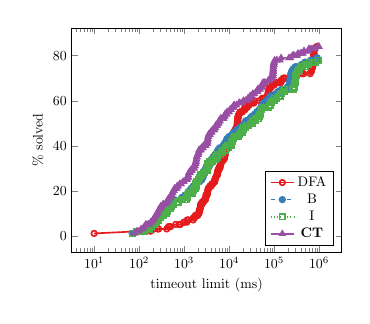
\begin{tikzpicture}[scale=0.5]
      \begin{axis}[
    xmode=log,
    every axis plot/.style={thin},
    xlabel={timeout limit (ms)},
    ylabel={\% solved},
    legend pos=south east,
    cycle list/Set1-6,
            % define fill color for the marker
            mark list fill={.!75!white},
            mark options={solid},
            cycle multiindex* list={
                Set1-6
                    \nextlist
                [3 of]linestyles
                    \nextlist
                very thick
                \nextlist
                mark=o,
                mark=*,
                mark=square,
                mark=triangle,
                mark=+
            },
    ]

    \addplot
    coordinates {
      (10, 1)
      (110, 2)
      (180, 2)
      (220, 3)
      (260, 3)
      (270, 3)
      (410, 3)
      (450, 4)
      (460, 4)
      (500, 4)
      (650, 5)
      (770, 5)
      (800, 5)
      (820, 5)
      (990, 6)
      (1010, 6)
      (1150, 6)
      (1180, 7)
      (1240, 7)
      (1590, 7)
      (1610, 8)
      (1650, 8)
      (1710, 8)
      (1770, 9)
      (1900, 9)
      (1960, 9)
      (2010, 9)
      (2100, 10)
      (2150, 10)
      (2160, 11)
      (2180, 11)
      (2220, 11)
      (2230, 12)
      (2290, 12)
      (2310, 13)
      (2320, 13)
      (2330, 14)
      (2420, 14)
      (2430, 14)
      (2500, 14)
      (2530, 15)
      (2680, 15)
      (2700, 15)
      (2830, 16)
      (2920, 16)
      (2980, 16)
      (3010, 17)
      (3030, 17)
      (3050, 18)
      (3200, 18)
      (3210, 18)
      (3240, 19)
      (3280, 19)
      (3320, 19)
      (3330, 20)
      (3400, 20)
      (3450, 21)
      (3480, 21)
      (3730, 22)
      (3760, 22)
      (3940, 22)
      (3990, 22)
      (4110, 23)
      (4290, 23)
      (4310, 23)
      (4640, 24)
      (4690, 24)
      (4750, 24)
      (4780, 24)
      (4820, 25)
      (4870, 25)
      (4880, 25)
      (5070, 26)
      (5080, 26)
      (5350, 27)
      (5360, 27)
      (5440, 27)
      (5500, 27)
      (5510, 28)
      (5530, 28)
      (5560, 28)
      (5590, 29)
      (5720, 29)
      (5810, 29)
      (5820, 29)
      (5890, 30)
      (5960, 30)
      (6220, 30)
      (6230, 31)
      (6250, 31)
      (6380, 31)
      (6440, 31)
      (6480, 32)
      (6520, 32)
      (6550, 32)
      (6570, 33)
      (6580, 33)
      (6800, 33)
      (7090, 33)
      (7260, 34)
      (7330, 34)
      (7780, 34)
      (7850, 35)
      (7880, 35)
      (7950, 35)
      (8040, 36)
      (8080, 36)
      (8120, 36)
      (8210, 37)
      (8220, 37)
      (8260, 37)
      (8270, 37)
      (8360, 38)
      (8610, 38)
      (8640, 38)
      (8680, 39)
      (8890, 39)
      (9010, 40)
      (9320, 40)
      (9340, 40)
      (9400, 40)
      (9680, 41)
      (9910, 41)
      (10500, 41)
      (10730, 42)
      (10750, 42)
      (11760, 42)
      (11790, 42)
      (11800, 43)
      (11860, 44)
      (11960, 44)
      (12080, 44)
      (12180, 44)
      (12200, 45)
      (12320, 45)
      (12380, 45)
      (12510, 46)
      (12890, 46)
      (13060, 46)
      (13420, 46)
      (13450, 47)
      (14040, 47)
      (14510, 47)
      (14650, 48)
      (14670, 48)
      (14920, 48)
      (14940, 48)
      (15080, 49)
      (15100, 49)
      (15160, 49)
      (15230, 50)
      (15340, 50)
      (15400, 50)
      (15430, 50)
      (15440, 51)
      (15460, 51)
      (15560, 52)
      (15580, 52)
      (15640, 52)
      (15710, 53)
      (16000, 53)
      (16010, 53)
      (16070, 53)
      (16460, 54)
      (16630, 54)
      (16680, 54)
      (17610, 55)
      (17890, 55)
      (19260, 55)
      (19840, 55)
      (22330, 56)
      (22400, 56)
      (22450, 57)
      (22550, 57)
      (22760, 57)
      (25190, 57)
      (26900, 58)
      (27380, 58)
      (27690, 58)
      (29920, 59)
      (32350, 59)
      (35390, 59)
      (35600, 59)
      (36330, 60)
      (47190, 60)
      (53920, 60)
      (54060, 61)
      (55680, 61)
      (57330, 61)
      (60090, 61)
      (69990, 62)
      (72350, 62)
      (73360, 62)
      (73510, 63)
      (73890, 63)
      (74370, 63)
      (74620, 64)
      (74690, 64)
      (75060, 64)
      (75610, 64)
      (76370, 65)
      (77380, 65)
      (77880, 65)
      (78820, 66)
      (79140, 66)
      (83730, 66)
      (86390, 66)
      (89030, 67)
      (91500, 67)
      (101460, 67)
      (110980, 68)
      (120070, 68)
      (131580, 68)
      (141010, 68)
      (142500, 69)
      (143660, 69)
      (149300, 69)
      (160480, 70)
      (169980, 70)
      (176980, 70)
      (238040, 70)
      (260120, 71)
      (280500, 71)
      (292530, 71)
      (400610, 72)
      (426190, 72)
      (453800, 72)
      (631530, 72)
      (663310, 73)
      (668120, 73)
      (674240, 73)
      (674950, 74)
      (681210, 74)
      (682080, 74)
      (693360, 74)
      (701800, 75)
      (710510, 75)
      (721370, 75)
      (724850, 76)
      (733270, 76)
      (737690, 76)
      (743100, 77)
      (744950, 77)
      (746390, 77)
      (747580, 77)
      (747780, 78)
      (749520, 78)
      (752380, 78)
      (752460, 79)
      (752970, 79)
      (756240, 79)
      (756590, 79)
      (757070, 80)
      (757940, 80)
      (757950, 80)
      (758210, 81)
      (760950, 81)
      (761150, 81)
      (761270, 81)
      (762350, 82)
      (764150, 82)
      (764630, 82)
      (766660, 83)
      (778590, 83)
      (779820, 83)
      (793780, 83)
      (874920, 84)
      
    };
    \addplot
    coordinates {
      (70, 1)
      (90, 2)
      (120, 2)
      (130, 3)
      (140, 4)
      (170, 4)
      (180, 4)
      (190, 4)
      (200, 5)
      (220, 6)
      (240, 7)
      (250, 7)
      (260, 8)
      (270, 8)
      (280, 8)
      (290, 8)
      (300, 9)
      (310, 9)
      (320, 10)
      (330, 10)
      (340, 10)
      (350, 11)
      (360, 12)
      (410, 12)
      (430, 12)
      (440, 13)
      (490, 13)
      (500, 13)
      (510, 14)
      (530, 14)
      (540, 14)
      (570, 15)
      (590, 15)
      (610, 16)
      (820, 16)
      (840, 16)
      (890, 17)
      (930, 17)
      (990, 17)
      (1000, 17)
      (1040, 18)
      (1140, 18)
      (1150, 18)
      (1160, 18)
      (1200, 19)
      (1230, 19)
      (1240, 19)
      (1250, 19)
      (1310, 20)
      (1330, 20)
      (1340, 20)
      (1430, 21)
      (1530, 21)
      (1550, 21)
      (1560, 21)
      (1590, 22)
      (1600, 22)
      (1770, 22)
      (1790, 23)
      (1860, 23)
      (1890, 23)
      (1930, 24)
      (1990, 24)
      (2150, 24)
      (2230, 24)
      (2380, 25)
      (2410, 25)
      (2470, 25)
      (2480, 25)
      (2490, 26)
      (2500, 26)
      (2540, 26)
      (2640, 26)
      (2650, 27)
      (2670, 27)
      (2680, 28)
      (2760, 28)
      (2810, 28)
      (2820, 29)
      (2900, 29)
      (2920, 29)
      (2940, 29)
      (3020, 30)
      (3060, 30)
      (3110, 30)
      (3150, 30)
      (3170, 31)
      (3180, 31)
      (3490, 31)
      (3690, 31)
      (3860, 32)
      (3870, 32)
      (3890, 32)
      (3980, 33)
      (3990, 33)
      (4020, 33)
      (4030, 34)
      (4110, 34)
      (4150, 34)
      (4310, 34)
      (4430, 35)
      (4500, 35)
      (4540, 35)
      (4570, 35)
      (4830, 36)
      (5260, 36)
      (5280, 36)
      (5300, 36)
      (5310, 37)
      (5340, 37)
      (5400, 37)
      (5650, 38)
      (5680, 38)
      (5800, 38)
      (5820, 38)
      (6110, 39)
      (6980, 39)
      (7080, 39)
      (7220, 39)
      (7400, 40)
      (7450, 40)
      (7810, 40)
      (7860, 41)
      (8060, 41)
      (8140, 41)
      (8430, 41)
      (8550, 42)
      (8620, 42)
      (8670, 42)
      (8910, 43)
      (9070, 43)
      (9370, 43)
      (9820, 44)
      (10010, 44)
      (11380, 44)
      (11530, 44)
      (11710, 45)
      (11730, 45)
      (11870, 45)
      (12640, 45)
      (12890, 46)
      (12980, 46)
      (13190, 46)
      (13360, 46)
      (14750, 47)
      (16070, 47)
      (16570, 47)
      (16890, 47)
      (17220, 48)
      (17390, 48)
      (19500, 48)
      (19830, 49)
      (20590, 49)
      (20970, 49)
      (21360, 49)
      (21880, 50)
      (22230, 50)
      (22410, 50)
      (22720, 50)
      (23330, 51)
      (23780, 51)
      (25040, 51)
      (26230, 51)
      (28680, 52)
      (29530, 52)
      (29620, 52)
      (29790, 52)
      (31460, 53)
      (34060, 53)
      (36050, 53)
      (36900, 54)
      (37690, 54)
      (38770, 54)
      (40250, 54)
      (41320, 55)
      (42030, 55)
      (42330, 55)
      (43940, 55)
      (46690, 56)
      (48760, 56)
      (48960, 56)
      (50130, 56)
      (50220, 57)
      (51730, 57)
      (52950, 57)
      (53130, 57)
      (53810, 58)
      (55650, 58)
      (56640, 58)
      (58080, 59)
      (61450, 59)
      (63420, 59)
      (63540, 59)
      (66170, 60)
      (71020, 60)
      (72660, 60)
      (76620, 60)
      (77150, 61)
      (78780, 61)
      (79600, 61)
      (81280, 61)
      (81780, 62)
      (82090, 62)
      (87960, 62)
      (99550, 62)
      (105960, 63)
      (111260, 63)
      (117310, 63)
      (119830, 63)
      (121100, 64)
      (124670, 64)
      (140000, 64)
      (144690, 65)
      (172980, 65)
      (182410, 65)
      (189610, 65)
      (196100, 66)
      (204580, 66)
      (211480, 66)
      (211610, 66)
      (214100, 67)
      (216690, 67)
      (218950, 67)
      (219710, 67)
      (221560, 68)
      (223130, 68)
      (225000, 68)
      (225250, 68)
      (226390, 69)
      (228770, 69)
      (228800, 69)
      (229210, 70)
      (229280, 70)
      (230400, 70)
      (230980, 70)
      (232150, 71)
      (236310, 71)
      (236880, 71)
      (237290, 72)
      (237320, 72)
      (238430, 72)
      (242000, 72)
      (245860, 73)
      (247080, 73)
      (253650, 73)
      (259880, 73)
      (262580, 74)
      (263130, 74)
      (290830, 74)
      (294050, 75)
      (300490, 75)
      (308680, 75)
      (373150, 75)
      (401120, 76)
      (417270, 76)
      (418050, 76)
      (460580, 76)
      (478710, 77)
      (486200, 77)
      (489550, 77)
      (539430, 77)
      (651220, 78)
      (786510, 78)
      (881100, 78)
      (882020, 78)
      (899860, 79)
      (908970, 79)
      
    };
    \addplot
    coordinates {
      (70, 1)
      (90, 2)
      (100, 2)
      (130, 2)
      (140, 3)
      (150, 3)
      (170, 3)
      (190, 4)
      (220, 5)
      (240, 6)
      (250, 7)
      (260, 7)
      (270, 7)
      (280, 8)
      (290, 8)
      (300, 8)
      (310, 9)
      (330, 9)
      (340, 9)
      (350, 9)
      (360, 10)
      (390, 10)
      (410, 10)
      (420, 11)
      (430, 11)
      (440, 12)
      (450, 12)
      (490, 12)
      (500, 13)
      (510, 13)
      (520, 13)
      (530, 14)
      (540, 14)
      (550, 14)
      (570, 14)
      (590, 15)
      (680, 15)
      (720, 15)
      (730, 15)
      (900, 16)
      (1040, 16)
      (1100, 16)
      (1120, 17)
      (1130, 17)
      (1160, 17)
      (1170, 18)
      (1180, 18)
      (1200, 18)
      (1280, 19)
      (1330, 19)
      (1400, 19)
      (1520, 19)
      (1570, 20)
      (1610, 20)
      (1620, 20)
      (1660, 21)
      (1710, 21)
      (1720, 21)
      (1740, 21)
      (1810, 22)
      (1830, 22)
      (1840, 23)
      (1860, 24)
      (1910, 24)
      (2020, 24)
      (2060, 25)
      (2070, 25)
      (2100, 25)
      (2130, 25)
      (2180, 26)
      (2220, 26)
      (2300, 27)
      (2480, 27)
      (2670, 28)
      (2690, 28)
      (2740, 28)
      (2870, 28)
      (3120, 29)
      (3130, 29)
      (3290, 29)
      (3300, 30)
      (3310, 30)
      (3330, 30)
      (3350, 30)
      (3370, 31)
      (3380, 31)
      (3390, 31)
      (3410, 32)
      (3580, 32)
      (3680, 32)
      (3710, 33)
      (3730, 33)
      (3870, 33)
      (4190, 33)
      (4380, 34)
      (4460, 34)
      (4940, 34)
      (4960, 35)
      (4980, 35)
      (5180, 35)
      (5500, 35)
      (5660, 36)
      (5750, 36)
      (6480, 36)
      (6820, 37)
      (7030, 37)
      (7220, 38)
      (8050, 38)
      (8060, 38)
      (8230, 38)
      (8390, 39)
      (9240, 39)
      (9260, 39)
      (9460, 39)
      (9470, 40)
      (9790, 40)
      (10460, 40)
      (11110, 40)
      (11190, 41)
      (11310, 41)
      (11340, 41)
      (11410, 41)
      (11530, 42)
      (11550, 42)
      (12070, 42)
      (12140, 42)
      (12400, 43)
      (12500, 43)
      (12540, 43)
      (13500, 44)
      (14750, 44)
      (15190, 44)
      (16340, 44)
      (16930, 45)
      (16950, 45)
      (17090, 45)
      (17130, 45)
      (17930, 46)
      (18320, 46)
      (19450, 46)
      (19470, 46)
      (19480, 47)
      (19510, 47)
      (19540, 47)
      (20450, 47)
      (21220, 48)
      (21880, 48)
      (23590, 48)
      (24380, 49)
      (25370, 49)
      (26140, 49)
      (26380, 49)
      (29480, 50)
      (31680, 50)
      (31710, 50)
      (33380, 50)
      (33770, 51)
      (34960, 51)
      (36010, 51)
      (37680, 51)
      (38200, 52)
      (43420, 52)
      (45490, 52)
      (45590, 52)
      (45940, 53)
      (47230, 53)
      (47430, 53)
      (47500, 54)
      (47910, 54)
      (48610, 54)
      (49700, 54)
      (49750, 55)
      (49820, 55)
      (49990, 55)
      (50810, 55)
      (50990, 56)
      (51050, 56)
      (51890, 56)
      (53250, 56)
      (54990, 57)
      (61930, 57)
      (64770, 57)
      (75650, 57)
      (80610, 58)
      (80830, 58)
      (82230, 58)
      (82650, 59)
      (84490, 59)
      (86990, 59)
      (87290, 59)
      (90540, 60)
      (91560, 60)
      (95830, 60)
      (100070, 60)
      (100420, 61)
      (101350, 61)
      (112290, 61)
      (113230, 61)
      (127520, 62)
      (130370, 62)
      (131320, 62)
      (136970, 62)
      (138480, 63)
      (140830, 63)
      (142650, 63)
      (148310, 63)
      (159010, 64)
      (159870, 64)
      (169450, 64)
      (170720, 65)
      (219870, 65)
      (259470, 65)
      (261960, 65)
      (266180, 66)
      (275900, 66)
      (277610, 66)
      (280260, 66)
      (282090, 67)
      (283200, 67)
      (283420, 67)
      (285910, 67)
      (287700, 68)
      (288220, 68)
      (291090, 68)
      (291560, 68)
      (294120, 69)
      (297560, 69)
      (297750, 69)
      (299160, 70)
      (300220, 70)
      (300620, 70)
      (301270, 70)
      (304330, 71)
      (308970, 71)
      (310620, 71)
      (310750, 71)
      (310990, 72)
      (311140, 72)
      (311540, 72)
      (315640, 72)
      (328920, 73)
      (329910, 73)
      (341360, 73)
      (344520, 73)
      (345500, 74)
      (351830, 74)
      (362040, 74)
      (382920, 75)
      (407830, 75)
      (434490, 75)
      (489800, 75)
      (494900, 76)
      (538120, 76)
      (565200, 76)
      (581200, 76)
      (605840, 77)
      (701390, 77)
      (717840, 77)
      (819870, 77)
      (958060, 78)
      
    };
    \addplot
    coordinates {
      (80, 1)
      (90, 2)
      (100, 2)
      (110, 3)
      (120, 3)
      (130, 4)
      (140, 5)
      (150, 5)
      (160, 5)
      (170, 5)
      (180, 6)
      (190, 6)
      (200, 7)
      (210, 7)
      (220, 8)
      (230, 9)
      (240, 9)
      (250, 10)
      (260, 10)
      (270, 11)
      (280, 12)
      (290, 12)
      (300, 13)
      (310, 13)
      (320, 13)
      (340, 14)
      (350, 14)
      (400, 14)
      (410, 15)
      (420, 15)
      (430, 16)
      (440, 16)
      (450, 16)
      (470, 17)
      (480, 17)
      (490, 17)
      (500, 17)
      (510, 18)
      (520, 18)
      (530, 18)
      (550, 19)
      (560, 19)
      (570, 20)
      (580, 20)
      (600, 20)
      (610, 21)
      (630, 21)
      (680, 21)
      (690, 21)
      (700, 22)
      (710, 22)
      (740, 22)
      (800, 23)
      (810, 23)
      (860, 23)
      (940, 24)
      (990, 24)
      (1090, 25)
      (1110, 25)
      (1160, 25)
      (1170, 25)
      (1220, 26)
      (1230, 26)
      (1240, 26)
      (1250, 27)
      (1270, 28)
      (1300, 28)
      (1350, 28)
      (1360, 28)
      (1390, 29)
      (1410, 29)
      (1430, 29)
      (1510, 29)
      (1530, 30)
      (1570, 30)
      (1650, 30)
      (1670, 30)
      (1700, 31)
      (1740, 31)
      (1750, 31)
      (1780, 32)
      (1810, 32)
      (1820, 33)
      (1830, 33)
      (1840, 33)
      (1870, 34)
      (1880, 34)
      (1890, 35)
      (1910, 35)
      (1920, 35)
      (1930, 35)
      (1980, 36)
      (2000, 36)
      (2030, 36)
      (2080, 36)
      (2090, 37)
      (2110, 37)
      (2130, 38)
      (2170, 38)
      (2200, 38)
      (2390, 38)
      (2410, 39)
      (2470, 39)
      (2530, 39)
      (2640, 39)
      (2680, 40)
      (2930, 40)
      (2990, 40)
      (3000, 40)
      (3100, 41)
      (3130, 41)
      (3200, 41)
      (3290, 41)
      (3310, 42)
      (3320, 42)
      (3330, 42)
      (3340, 43)
      (3360, 43)
      (3370, 43)
      (3410, 44)
      (3440, 44)
      (3480, 44)
      (3500, 45)
      (3540, 45)
      (3710, 45)
      (3760, 45)
      (3870, 46)
      (3920, 46)
      (3990, 46)
      (4120, 46)
      (4240, 47)
      (4360, 47)
      (4650, 47)
      (4760, 47)
      (4800, 48)
      (4960, 48)
      (5030, 49)
      (5160, 49)
      (5340, 49)
      (5480, 49)
      (5640, 50)
      (5650, 50)
      (5810, 50)
      (5870, 50)
      (5960, 51)
      (6020, 51)
      (6220, 51)
      (6250, 51)
      (6430, 52)
      (6560, 52)
      (6900, 52)
      (7590, 52)
      (7710, 53)
      (7920, 53)
      (7990, 53)
      (8070, 54)
      (8460, 54)
      (8610, 54)
      (8860, 54)
      (8910, 55)
      (9510, 55)
      (9780, 55)
      (10050, 55)
      (10460, 56)
      (10710, 56)
      (10930, 56)
      (11000, 56)
      (11810, 57)
      (11830, 57)
      (11850, 57)
      (12690, 57)
      (12730, 58)
      (13290, 58)
      (14610, 58)
      (16570, 59)
      (17080, 59)
      (17280, 59)
      (19780, 59)
      (20620, 60)
      (22880, 60)
      (23710, 60)
      (25350, 60)
      (26090, 61)
      (26760, 61)
      (28670, 61)
      (28700, 61)
      (29110, 62)
      (30440, 62)
      (30960, 62)
      (31500, 62)
      (33570, 63)
      (33600, 63)
      (33980, 63)
      (36670, 63)
      (40260, 64)
      (42020, 64)
      (42870, 64)
      (42900, 65)
      (43980, 65)
      (44870, 65)
      (48890, 65)
      (49710, 66)
      (52440, 66)
      (52780, 66)
      (53490, 66)
      (54330, 67)
      (54840, 67)
      (55390, 67)
      (55780, 67)
      (56350, 68)
      (59620, 68)
      (62080, 68)
      (63030, 68)
      (74100, 69)
      (76760, 69)
      (77540, 69)
      (82360, 70)
      (82400, 70)
      (89920, 70)
      (92730, 70)
      (93300, 71)
      (93750, 71)
      (93760, 71)
      (93770, 71)
      (93910, 72)
      (94080, 72)
      (94150, 72)
      (94190, 72)
      (94750, 73)
      (95060, 73)
      (95240, 73)
      (95480, 73)
      (95620, 74)
      (95790, 74)
      (95950, 74)
      (96350, 75)
      (96460, 75)
      (96710, 75)
      (97070, 76)
      (97530, 76)
      (98260, 76)
      (98700, 76)
      (99170, 77)
      (99350, 77)
      (99830, 77)
      (100100, 77)
      (102440, 78)
      (114340, 78)
      (115600, 78)
      (135440, 78)
      (142690, 79)
      (213710, 79)
      (232160, 79)
      (256150, 80)
      (269010, 80)
      (286750, 80)
      (326240, 80)
      (337620, 81)
      (382900, 81)
      (409250, 81)
      (436840, 81)
      (459860, 82)
      (466130, 82)
      (579410, 82)
      (588000, 82)
      (591240, 83)
      (628380, 83)
      (694360, 83)
      (805460, 83)
      (942180, 84)
      (958960, 84)
      (984010, 84)
      (995270, 84)
      
    };
    

    \legend{ DFA, B, I, \textbf{CT} }
  \end{axis}

    \end{tikzpicture} 
    
    \bigskip
    
    \small
    $661$ instances after filtering out those where
    \begin{itemize}
      \item the runtime was~$< 1$ s for all algorithm ($639$~instances), or
      \item at least one algorithm ran out of memory ($207$~instances).
    \end{itemize}

\end{frame}

\begin{frame}
  \frametitle{Small tables}
  \framesubtitle{$3-7$~tuples}
  \begin{tabular}{cc}
      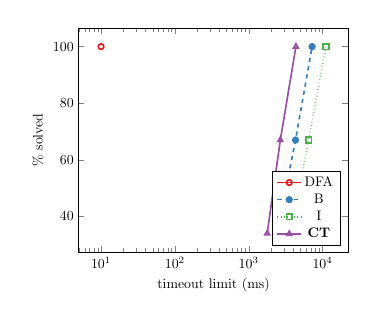
\begin{tikzpicture}[scale=0.5]
        \begin{axis}[
    xmode=log,
    every axis plot/.style={thin},
    xlabel={timeout limit (ms)},
    ylabel={\% solved},
    legend pos=south east,
    cycle list/Set1-6,
            % define fill color for the marker
            mark list fill={.!75!white},
            mark options={solid},
            cycle multiindex* list={
                Set1-6
                    \nextlist
                [3 of]linestyles
                    \nextlist
                very thick
                \nextlist
                mark=o,
                mark=*,
                mark=square,
                mark=triangle,
                mark=+
            },
    ]

    \addplot
    coordinates {
      (10, 100)
      
    };
    \addplot
    coordinates {
      (2410, 34)
      (4310, 67)
      (7220, 100)
      
    };
    \addplot
    coordinates {
      (3730, 34)
      (6480, 67)
      (11110, 100)
      
    };
    \addplot
    coordinates {
      (1780, 34)
      (2680, 67)
      (4360, 100)
      
    };
    

    \legend{ DFA, B, I, \textbf{CT} }
  \end{axis}

      \end{tikzpicture} 
    &
    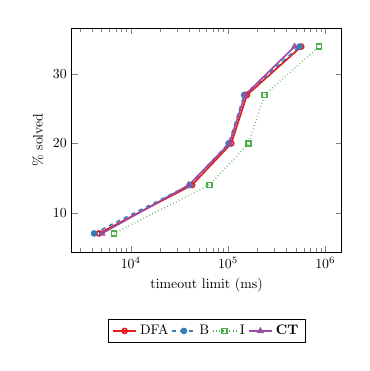
\begin{tikzpicture}[scale=0.5]
      \begin{axis}[
    xmode=log,
    every axis plot/.style={thin},
    xlabel={timeout limit (ms)},
    ylabel={\% solved},
    legend style={at={(0.5,-0.30)},
      anchor=north,legend columns=-1},
    % legend pos=south east,
    cycle list/Set1-6,
            % define fill color for the marker
            mark list fill={.!75!white},
            mark options={solid,scale=0.9},
            cycle multiindex* list={
                Set1-6
                    \nextlist
                [3 of]linestyles
                    \nextlist
                very thick
                \nextlist
                mark=o,
                mark=*,
                mark=square,
                mark=triangle,
                mark=+
            },
    ]

    \addplot
    coordinates {
      (4710, 7)
      (42720, 14)
      (107940, 20)
      (156470, 27)
      (565750, 34)
      
    };
    \addplot
    coordinates {
      (4200, 7)
      (40280, 14)
      (101330, 20)
      (146750, 27)
      (542500, 34)
      
    };
    \addplot
    coordinates {
      (6700, 7)
      (64020, 14)
      (162760, 20)
      (236800, 27)
      (861730, 34)
      
    };
    \addplot
    coordinates {
      (5070, 7)
      (39550, 14)
      (103230, 20)
      (149210, 27)
      (482760, 34)
      
    };
    

    \legend{ DFA, B, I, \textbf{CT} }
  \end{axis}

    \end{tikzpicture} \\
    
    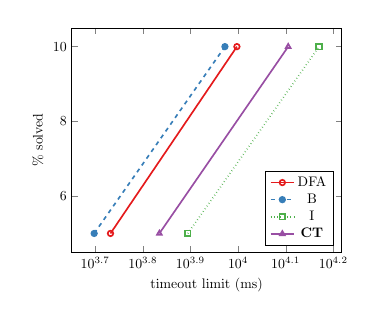
\begin{tikzpicture}[scale=0.5]
      \begin{axis}[
    xmode=log,
    every axis plot/.style={thin},
    xlabel={timeout limit (ms)},
    ylabel={\% solved},
    legend pos=south east,
    cycle list/Set1-6,
            % define fill color for the marker
            mark list fill={.!75!white},
            mark options={solid},
            cycle multiindex* list={
                Set1-6
                    \nextlist
                [3 of]linestyles
                    \nextlist
                very thick
                \nextlist
                mark=o,
                mark=*,
                mark=square,
                mark=triangle,
                mark=+
            },
    ]

    \addplot
    coordinates {
      (5400, 5)
      (9950, 10)
      
    };
    \addplot
    coordinates {
      (4990, 5)
      (9390, 10)
      
    };
    \addplot
    coordinates {
      (7850, 5)
      (14800, 10)
      
    };
    \addplot
    coordinates {
      (6840, 5)
      (12750, 10)
      
    };
    

    \legend{ DFA, B, I, \textbf{CT} }
  \end{axis}

    \end{tikzpicture} & 
        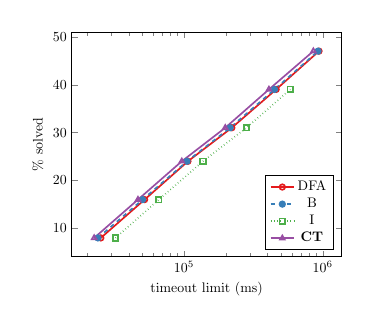
\begin{tikzpicture}[scale=0.5]
      \begin{axis}[
    xmode=log,
    every axis plot/.style={thin},
    xlabel={timeout limit (ms)},
    ylabel={\% solved},
    legend pos=south east,
    cycle list/Set1-6,
            % define fill color for the marker
            mark list fill={.!75!white},
            mark options={solid},
            cycle multiindex* list={
                Set1-6
                    \nextlist
                [3 of]linestyles
                    \nextlist
                very thick
                \nextlist
                mark=o,
                mark=*,
                mark=square,
                mark=triangle,
                mark=+
            },
    ]

    \addplot
    coordinates {
      (25170, 8)
      (52050, 16)
      (106800, 24)
      (221140, 31)
      (461470, 39)
      (939670, 47)
      
    };
    \addplot
    coordinates {
      (23990, 8)
      (50380, 16)
      (105170, 24)
      (215170, 31)
      (449310, 39)
      (925510, 47)
      
    };
    \addplot
    coordinates {
      (32120, 8)
      (65960, 16)
      (137030, 24)
      (282220, 31)
      (583270, 39)
      
    };
    \addplot
    coordinates {
      (22530, 8)
      (46610, 16)
      (96430, 24)
      (198370, 31)
      (409390, 39)
      (855630, 47)
      
    };
    

    \legend{ DFA, B, I, \textbf{CT} }
  \end{axis}

    \end{tikzpicture} \\

  \end{tabular}
\end{frame}

\begin{frame}
  \frametitle{Large tables}
  \framesubtitle{$2500-10000$~tuples}
  \begin{tabular}{cc}
    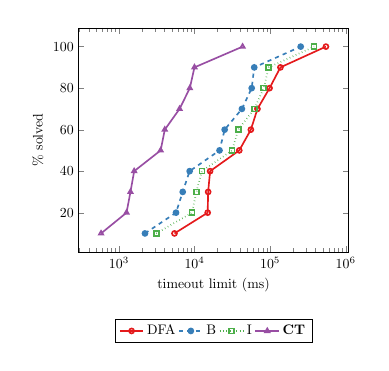
\begin{tikzpicture}[scale=0.5]
      \begin{axis}[
    xmode=log,
    every axis plot/.style={thin},
    xlabel={timeout limit (ms)},
    ylabel={\% solved},
    legend style={at={(0.5,-0.30)},
      anchor=north,legend columns=-1},
    % legend pos=south east,
    cycle list/Set1-6,
            % define fill color for the marker
            mark list fill={.!75!white},
            mark options={solid,scale=0.9},
            cycle multiindex* list={
                Set1-6
                    \nextlist
                [3 of]linestyles
                    \nextlist
                very thick
                \nextlist
                mark=o,
                mark=*,
                mark=square,
                mark=triangle,
                mark=+
            },
    ]

    \addplot
    coordinates {
      (5430, 10)
      (14920, 20)
      (15140, 30)
      (16070, 40)
      (39070, 50)
      (55650, 60)
      (68040, 70)
      (98270, 80)
      (136850, 90)
      (547470, 100)
      
    };
    \addplot
    coordinates {
      (2210, 10)
      (5690, 20)
      (6980, 30)
      (8620, 40)
      (21410, 50)
      (25040, 60)
      (42340, 70)
      (57090, 80)
      (61660, 90)
      (253910, 100)
      
    };
    \addplot
    coordinates {
      (3120, 10)
      (9260, 20)
      (10590, 30)
      (12520, 40)
      (31430, 50)
      (37860, 60)
      (61840, 70)
      (82360, 80)
      (95870, 90)
      (382470, 100)
      
    };
    \addplot
    coordinates {
      (580, 10)
      (1260, 20)
      (1420, 30)
      (1590, 40)
      (3560, 50)
      (4040, 60)
      (6340, 70)
      (8660, 80)
      (9980, 90)
      (43230, 100)
      
    };
    

    \legend{ DFA, B, I, \textbf{CT} }
  \end{axis}

    \end{tikzpicture}
    &
      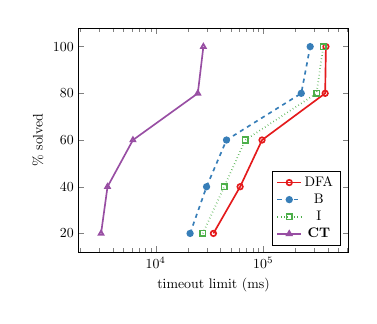
\begin{tikzpicture}[scale=0.5]
        \begin{axis}[
    xmode=log,
    every axis plot/.style={thin},
    xlabel={timeout limit (ms)},
    ylabel={\% solved},
    legend pos=south east,
    cycle list/Set1-6,
            % define fill color for the marker
            mark list fill={.!75!white},
            mark options={solid},
            cycle multiindex* list={
                Set1-6
                    \nextlist
                [3 of]linestyles
                    \nextlist
                very thick
                \nextlist
                mark=o,
                mark=*,
                mark=square,
                mark=triangle,
                mark=+
            },
    ]

    \addplot
    coordinates {
      (34430, 20)
      (60980, 40)
      (97460, 60)
      (376360, 80)
      (382430, 100)
      
    };
    \addplot
    coordinates {
      (20900, 20)
      (29740, 40)
      (45540, 60)
      (225660, 80)
      (273020, 100)
      
    };
    \addplot
    coordinates {
      (27430, 20)
      (43410, 40)
      (68070, 60)
      (313020, 80)
      (361180, 100)
      
    };
    \addplot
    coordinates {
      (3110, 20)
      (3570, 40)
      (6150, 60)
      (24650, 80)
      (27780, 100)
      
    };
    

    \legend{ DFA, B, I, \textbf{CT} }
  \end{axis}

      \end{tikzpicture} \\
    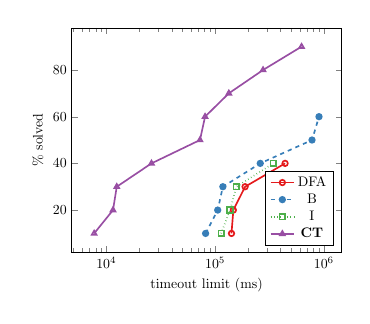
\begin{tikzpicture}[scale=0.5]
      \begin{axis}[
    xmode=log,
    every axis plot/.style={thin},
    xlabel={timeout limit (ms)},
    ylabel={\% solved},
    legend pos=south east,
    cycle list/Set1-6,
            % define fill color for the marker
            mark list fill={.!75!white},
            mark options={solid},
            cycle multiindex* list={
                Set1-6
                    \nextlist
                [3 of]linestyles
                    \nextlist
                very thick
                \nextlist
                mark=o,
                mark=*,
                mark=square,
                mark=triangle,
                mark=+
            },
    ]

    \addplot
    coordinates {
      (141410, 10)
      (147100, 20)
      (188630, 30)
      (439630, 40)
      
    };
    \addplot
    coordinates {
      (81770, 10)
      (105640, 20)
      (117810, 30)
      (259930, 40)
      (777770, 50)
      (901390, 60)
      
    };
    \addplot
    coordinates {
      (113550, 10)
      (137140, 20)
      (156920, 30)
      (342630, 40)
      
    };
    \addplot
    coordinates {
      (7730, 10)
      (11520, 20)
      (12470, 30)
      (26010, 40)
      (72590, 50)
      (80830, 60)
      (133710, 70)
      (275860, 80)
      (623230, 90)
      
    };
    

    \legend{ DFA, B, I, \textbf{CT} }
  \end{axis}

    \end{tikzpicture}
    &
      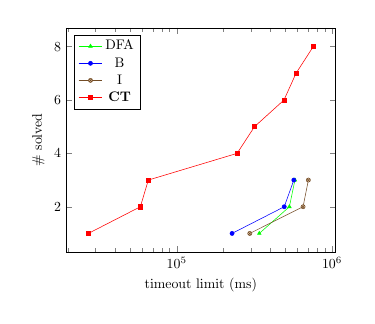
\begin{tikzpicture}[scale=0.5]
        \begin{axis}[
    xmode=log,
    every axis plot/.style={thin},
    xlabel={timeout limit (ms)},
    ylabel={\# solved},
    legend pos=north west
    % table/create on use/cumulative distribution/.style={
    %   create col/expr={\pgfmathaccuma + \thisrow{f(x)}}   
    % }
    ]
    \addplot 
    [mark=triangle*,
    mark size=1.5,
    mark options={solid},
    green] 
    coordinates {
    (339960.449, 1)
(531357.500, 2)
(576758.002, 3)
% (1006830.253, 4)
% (1006953.686, 5)
% (1006987.278, 6)
% (1007012.182, 7)
% (1007040.479, 8)
% (1007166.422, 9)
% (1007385.382, 10)
    };

    \addplot 
    [blue,
    mark=*,
    mark size=1.5,
    mark options={solid}]
    coordinates {
    (227052.199, 1)
(492242.811, 2)
(567372.313, 3)
% (1000877.234, 4)
% (1000889.042, 5)
% (1000892.874, 6)
% (1000895.207, 7)
% (1000911.856, 8)
% (1000913.878, 9)
% (1000928.789, 10)
    };

    \addplot [brown!60!black,
    mark options={fill=brown!40},
    mark=otimes*,
    mark size=1.5]
    coordinates {
    (295287.152, 1)
(650810.991, 2)
(703794.608, 3)
% (1000887.426, 4)
% (1000895.815, 5)
% (1000897.600, 6)
% (1000901.551, 7)
% (1000905.923, 8)
% (1000907.888, 9)
% (1000913.436, 10)
    };

    \addplot 
    [red,
    mark size=1.5,
    mark=square*]
    coordinates {
    (26984.703, 1)
(58304.179, 2)
(65624.179, 3)
(244616.117, 4)
(316746.918, 5)
(490346.243, 6)
(586068.768, 7)
(756641.057, 8)
%(1001171.576, 9)
%(1001192.839, 10)
    };
    \legend{DFA,B,I,\textbf{CT}}
  \end{axis}

      \end{tikzpicture} \\
  \end{tabular}
\end{frame}

\begin{frame}
  \frametitle{Large tables}
  \framesubtitle{$> 12000$~tuples}
  \begin{tabular}{cc}
    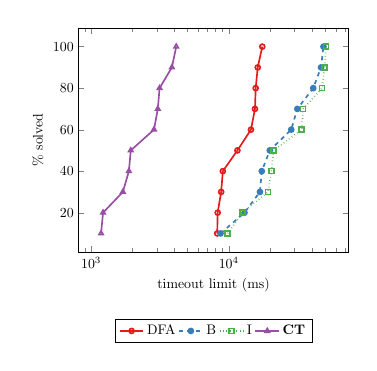
\begin{tikzpicture}[scale=0.5]
      \begin{axis}[
    xmode=log,
    every axis plot/.style={thin},
    xlabel={timeout limit (ms)},
    ylabel={\% solved},
    legend style={at={(0.5,-0.30)},
      anchor=north,legend columns=-1},
    % legend pos=south east,
    cycle list/Set1-6,
            % define fill color for the marker
            mark list fill={.!75!white},
            mark options={solid,scale=0.9},
            cycle multiindex* list={
                Set1-6
                    \nextlist
                [3 of]linestyles
                    \nextlist
                very thick
                \nextlist
                mark=o,
                mark=*,
                mark=square,
                mark=triangle,
                mark=+
            },
    ]

    \addplot
    coordinates {
      (8240, 10)
      (8300, 20)
      (8800, 30)
      (9050, 40)
      (11550, 50)
      (14490, 60)
      (15490, 70)
      (15680, 80)
      (16230, 90)
      (17510, 100)
      
    };
    \addplot
    coordinates {
      (8710, 10)
      (13000, 20)
      (16840, 30)
      (17370, 40)
      (19860, 50)
      (28430, 60)
      (31470, 70)
      (41080, 80)
      (46790, 90)
      (48720, 100)
      
    };
    \addplot
    coordinates {
      (9810, 10)
      (12550, 20)
      (19300, 30)
      (20370, 40)
      (21220, 50)
      (33870, 60)
      (34700, 70)
      (47590, 80)
      (49800, 90)
      (50780, 100)
      
    };
    \addplot
    coordinates {
      (1180, 10)
      (1220, 20)
      (1700, 30)
      (1880, 40)
      (1940, 50)
      (2860, 60)
      (3050, 70)
      (3140, 80)
      (3860, 90)
      (4150, 100)
      
    };
    

    \legend{ DFA, B, I, \textbf{CT} }
  \end{axis}

    \end{tikzpicture}
    &
      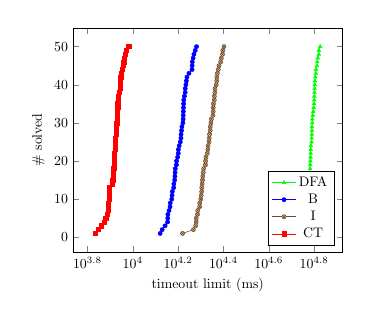
\begin{tikzpicture}[scale=0.5]
        \begin{axis}[
    xmode=log,
    every axis plot/.style={thin},
    xlabel={timeout limit (ms)},
    ylabel={\# solved},
    legend pos=south east
    % table/create on use/cumulative distribution/.style={
    %   create col/expr={\pgfmathaccuma + \thisrow{f(x)}}   
    % }
    ]
    \addplot 
    [mark=triangle*,
    mark size=1.5,
    mark options={solid},
    green] 
    coordinates {
    (51125.785, 1)
(54263.257, 2)
(56487.527, 3)
(56702.786, 4)
(56985.792, 5)
(57276.885, 6)
(57622.584, 7)
(58132.270, 8)
(58140.300, 9)
(58355.175, 10)
(58676.203, 11)
(59158.883, 12)
(59632.816, 13)
(59713.900, 14)
(59728.215, 15)
(60269.934, 16)
(60313.648, 17)
(60549.505, 18)
(60622.637, 19)
(60711.449, 20)
(60810.980, 21)
(60862.784, 22)
(60914.293, 23)
(61100.454, 24)
(61428.994, 25)
(61523.477, 26)
(61625.366, 27)
(61712.915, 28)
(61729.236, 29)
(61886.596, 30)
(61900.845, 31)
(62341.893, 32)
(62455.546, 33)
(62817.572, 34)
(63010.646, 35)
(63184.232, 36)
(63221.376, 37)
(63304.994, 38)
(63379.424, 39)
(63540.272, 40)
(63613.419, 41)
(63781.589, 42)
(64128.455, 43)
(64263.902, 44)
(64924.220, 45)
(65113.900, 46)
(65508.695, 47)
(66133.866, 48)
(66157.482, 49)
(67076.860, 50)
    };

    \addplot 
    [blue,
    mark=*,
    mark size=1.5,
    mark options={solid}]
    coordinates {
    (13210.645, 1)
(13478.699, 2)
(13880.904, 3)
(14240.906, 4)
(14262.586, 5)
(14281.012, 6)
(14453.879, 7)
(14601.257, 8)
(14630.915, 9)
(14856.229, 10)
(14906.587, 11)
(14947.426, 12)
(15147.432, 13)
(15173.599, 14)
(15300.351, 15)
(15338.350, 16)
(15370.471, 17)
(15400.162, 18)
(15575.398, 19)
(15599.555, 20)
(15767.367, 21)
(15876.487, 22)
(15890.540, 23)
(16026.936, 24)
(16207.081, 25)
(16313.213, 26)
(16328.178, 27)
(16410.911, 28)
(16468.425, 29)
(16641.910, 30)
(16678.794, 31)
(16689.212, 32)
(16716.749, 33)
(16728.322, 34)
(16755.929, 35)
(16780.814, 36)
(16896.779, 37)
(17026.619, 38)
(17037.921, 39)
(17147.387, 40)
(17237.324, 41)
(17326.549, 42)
(17685.575, 43)
(18266.956, 44)
(18281.157, 45)
(18310.293, 46)
(18466.165, 47)
(18608.783, 48)
(18864.433, 49)
(19102.683, 50)
    };

    \addplot [brown!60!black,
    mark options={fill=brown!40},
    mark=otimes*,
    mark size=1.5]
    coordinates {
    (16575.843, 1)
(18505.000, 2)
(18940.008, 3)
(19038.980, 4)
(19049.304, 5)
(19298.221, 6)
(19348.596, 7)
(19719.698, 8)
(19737.753, 9)
(19947.661, 10)
(20036.932, 11)
(20122.714, 12)
(20152.397, 13)
(20232.116, 14)
(20302.198, 15)
(20360.843, 16)
(20458.853, 17)
(20543.247, 18)
(20924.864, 19)
(20941.580, 20)
(21033.055, 21)
(21323.434, 22)
(21424.912, 23)
(21488.205, 24)
(21690.524, 25)
(21732.563, 26)
(21805.424, 27)
(21961.943, 28)
(21968.175, 29)
(22103.640, 30)
(22217.515, 31)
(22576.655, 32)
(22629.332, 33)
(22640.426, 34)
(22690.290, 35)
(22898.044, 36)
(22906.588, 37)
(23018.632, 38)
(23049.661, 39)
(23346.986, 40)
(23464.371, 41)
(23482.242, 42)
(23611.320, 43)
(23844.593, 44)
(24011.531, 45)
(24420.146, 46)
(24590.635, 47)
(24882.878, 48)
(24954.062, 49)
(25252.813, 50)
    };

    \addplot 
    [red,
    mark size=1.5,
    mark=square*]
    coordinates {
    (6834.272, 1)
(7049.566, 2)
(7238.120, 3)
(7457.754, 4)
(7598.772, 5)
(7739.737, 6)
(7771.586, 7)
(7772.970, 8)
(7812.433, 9)
(7861.439, 10)
(7862.003, 11)
(7867.552, 12)
(7871.233, 13)
(8146.006, 14)
(8162.853, 15)
(8169.022, 16)
(8197.217, 17)
(8246.900, 18)
(8258.157, 19)
(8262.374, 20)
(8291.516, 21)
(8318.251, 22)
(8342.451, 23)
(8355.561, 24)
(8389.425, 25)
(8401.690, 26)
(8470.665, 27)
(8475.034, 28)
(8489.871, 29)
(8495.761, 30)
(8507.506, 31)
(8510.152, 32)
(8560.945, 33)
(8587.622, 34)
(8588.072, 35)
(8642.789, 36)
(8662.209, 37)
(8738.285, 38)
(8798.802, 39)
(8820.422, 40)
(8831.432, 41)
(8851.771, 42)
(8928.438, 43)
(8949.293, 44)
(9107.856, 45)
(9118.812, 46)
(9135.516, 47)
(9225.896, 48)
(9370.806, 49)
(9607.234, 50)
    };
    \legend{DFA,B,I,CT}
  \end{axis}

      \end{tikzpicture} \\
    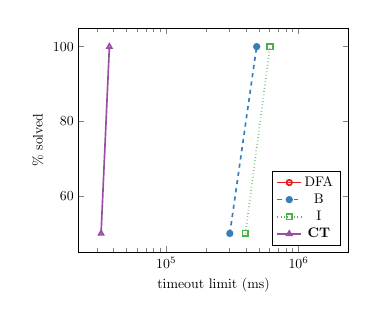
\begin{tikzpicture}[scale=0.5]
      \begin{axis}[
    xmode=log,
    every axis plot/.style={thin},
    xlabel={timeout limit (ms)},
    ylabel={\% solved},
    legend pos=south east,
    cycle list/Set1-6,
            % define fill color for the marker
            mark list fill={.!75!white},
            mark options={solid},
            cycle multiindex* list={
                Set1-6
                    \nextlist
                [3 of]linestyles
                    \nextlist
                very thick
                \nextlist
                mark=o,
                mark=*,
                mark=square,
                mark=triangle,
                mark=+
            },
    ]

    \addplot
    coordinates {
      (1609830, 50)
      
    };
    \addplot
    coordinates {
      (302190, 50)
      (482210, 100)
      
    };
    \addplot
    coordinates {
      (396530, 50)
      (608250, 100)
      
    };
    \addplot
    coordinates {
      (32160, 50)
      (37170, 100)
      
    };
    

    \legend{ DFA, B, I, \textbf{CT} }
  \end{axis}

    \end{tikzpicture}
    &
      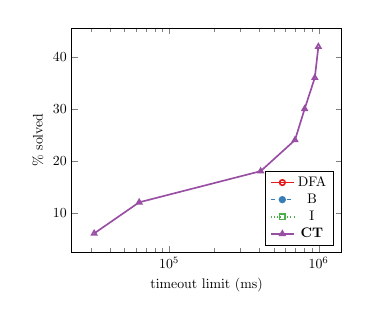
\begin{tikzpicture}[scale=0.5]
        \begin{axis}[
    xmode=log,
    every axis plot/.style={thin},
    xlabel={timeout limit (ms)},
    ylabel={\% solved},
    legend pos=south east,
    cycle list/Set1-6,
            % define fill color for the marker
            mark list fill={.!75!white},
            mark options={solid},
            cycle multiindex* list={
                Set1-6
                    \nextlist
                [3 of]linestyles
                    \nextlist
                very thick
                \nextlist
                mark=o,
                mark=*,
                mark=square,
                mark=triangle,
                mark=+
            },
    ]

    \addplot
    coordinates {
      (674950, 6)
      
    };
    \addplot
    coordinates {
      (1005060, 6)
      
    };
    \addplot
    coordinates {
      (1005070, 6)
      
    };
    \addplot
    coordinates {
      (31500, 6)
      (63030, 12)
      (409250, 18)
      (694360, 24)
      (805460, 30)
      (942180, 36)
      (995270, 42)
      
    };
    

    \legend{ DFA, B, I, \textbf{CT} }
  \end{axis}

      \end{tikzpicture} \\
  \end{tabular}
\end{frame}

\begin{frame}
  \frametitle{Low arities}
  \framesubtitle{$2-3$~variables}
  \begin{tabular}{cc}
    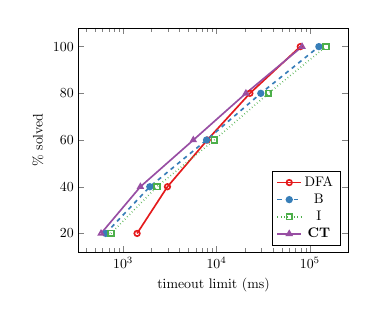
\begin{tikzpicture}[scale=0.5]
      \begin{axis}[
    xmode=log,
    every axis plot/.style={thin},
    xlabel={timeout limit (ms)},
    ylabel={\% solved},
    legend pos=south east,
    cycle list/Set1-6,
            % define fill color for the marker
            mark list fill={.!75!white},
            mark options={solid},
            cycle multiindex* list={
                Set1-6
                    \nextlist
                [3 of]linestyles
                    \nextlist
                very thick
                \nextlist
                mark=o,
                mark=*,
                mark=square,
                mark=triangle,
                mark=+
            },
    ]

    \addplot
    coordinates {
      (1410, 20)
      (2980, 40)
      (7950, 60)
      (22760, 80)
      (78820, 100)
      
    };
    \addplot
    coordinates {
      (650, 20)
      (1930, 40)
      (7810, 60)
      (29790, 80)
      (124670, 100)
      
    };
    \addplot
    coordinates {
      (740, 20)
      (2300, 40)
      (9460, 60)
      (36010, 80)
      (148310, 100)
      
    };
    \addplot
    coordinates {
      (580, 20)
      (1530, 40)
      (5640, 60)
      (20620, 80)
      (82360, 100)
      
    };
    

    \legend{ DFA, B, I, \textbf{CT} }
  \end{axis}

    \end{tikzpicture}
    &
      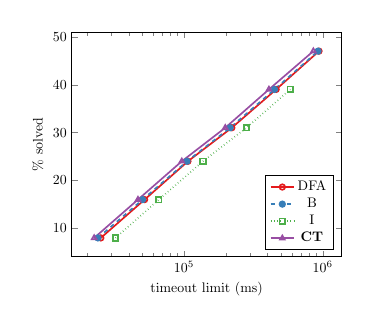
\begin{tikzpicture}[scale=0.5]
        \begin{axis}[
    xmode=log,
    every axis plot/.style={thin},
    xlabel={timeout limit (ms)},
    ylabel={\% solved},
    legend pos=south east,
    cycle list/Set1-6,
            % define fill color for the marker
            mark list fill={.!75!white},
            mark options={solid},
            cycle multiindex* list={
                Set1-6
                    \nextlist
                [3 of]linestyles
                    \nextlist
                very thick
                \nextlist
                mark=o,
                mark=*,
                mark=square,
                mark=triangle,
                mark=+
            },
    ]

    \addplot
    coordinates {
      (25170, 8)
      (52050, 16)
      (106800, 24)
      (221140, 31)
      (461470, 39)
      (939670, 47)
      
    };
    \addplot
    coordinates {
      (23990, 8)
      (50380, 16)
      (105170, 24)
      (215170, 31)
      (449310, 39)
      (925510, 47)
      
    };
    \addplot
    coordinates {
      (32120, 8)
      (65960, 16)
      (137030, 24)
      (282220, 31)
      (583270, 39)
      
    };
    \addplot
    coordinates {
      (22530, 8)
      (46610, 16)
      (96430, 24)
      (198370, 31)
      (409390, 39)
      (855630, 47)
      
    };
    

    \legend{ DFA, B, I, \textbf{CT} }
  \end{axis}

      \end{tikzpicture} \\
    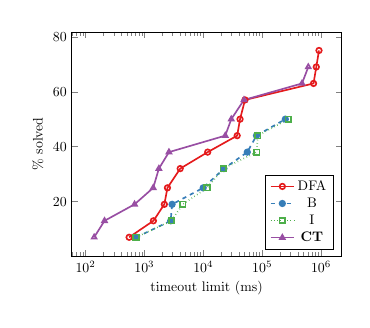
\begin{tikzpicture}[scale=0.5]
      \begin{axis}[
    xmode=log,
    every axis plot/.style={thin},
    xlabel={timeout limit (ms)},
    ylabel={\% solved},
    legend pos=south east,
    cycle list/Set1-6,
            % define fill color for the marker
            mark list fill={.!75!white},
            mark options={solid},
            cycle multiindex* list={
                Set1-6
                    \nextlist
                [3 of]linestyles
                    \nextlist
                very thick
                \nextlist
                mark=o,
                mark=*,
                mark=square,
                mark=triangle,
                mark=+
            },
    ]

    \addplot
    coordinates {
      (550, 7)
      (1420, 13)
      (2180, 19)
      (2460, 25)
      (4050, 32)
      (11860, 38)
      (37590, 44)
      (42030, 50)
      (51040, 57)
      (744510, 63)
      (828510, 69)
      (921350, 75)
      
    };
    \addplot
    coordinates {
      (730, 7)
      (2790, 13)
      (2950, 19)
      (9950, 25)
      (22390, 32)
      (55820, 38)
      (79890, 44)
      (247070, 50)
      
    };
    \addplot
    coordinates {
      (720, 7)
      (2880, 13)
      (4460, 19)
      (11570, 25)
      (21880, 32)
      (80590, 38)
      (84470, 44)
      (276470, 50)
      
    };
    \addplot
    coordinates {
      (140, 7)
      (210, 13)
      (680, 19)
      (1410, 25)
      (1760, 32)
      (2610, 38)
      (23590, 44)
      (29830, 50)
      (49050, 57)
      (474090, 63)
      (606460, 69)
      
    };
    

    \legend{ DFA, B, I, \textbf{CT} }
  \end{axis}

    \end{tikzpicture}
    &
      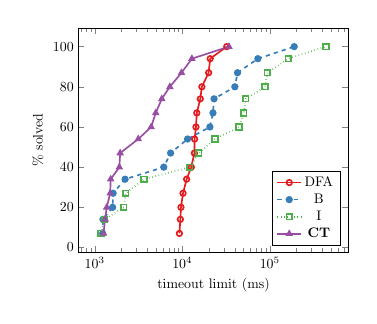
\begin{tikzpicture}[scale=0.5]
        \begin{axis}[
    xmode=log,
    every axis plot/.style={thin},
    xlabel={timeout limit (ms)},
    ylabel={\% solved},
    legend pos=south east,
    cycle list/Set1-6,
            % define fill color for the marker
            mark list fill={.!75!white},
            mark options={solid},
            cycle multiindex* list={
                Set1-6
                    \nextlist
                [3 of]linestyles
                    \nextlist
                very thick
                \nextlist
                mark=o,
                mark=*,
                mark=square,
                mark=triangle,
                mark=+
            },
    ]

    \addplot
    coordinates {
      (9270, 7)
      (9500, 14)
      (9650, 20)
      (10200, 27)
      (11200, 34)
      (12670, 40)
      (13740, 47)
      (13820, 54)
      (14320, 60)
      (14650, 67)
      (16050, 74)
      (16730, 80)
      (19980, 87)
      (20820, 94)
      (32170, 100)
      
    };
    \addplot
    coordinates {
      (1230, 7)
      (1240, 14)
      (1600, 20)
      (1620, 27)
      (2220, 34)
      (6140, 40)
      (7350, 47)
      (11490, 54)
      (20670, 60)
      (22400, 67)
      (23060, 74)
      (39870, 80)
      (42730, 87)
      (72970, 94)
      (189860, 100)
      
    };
    \addplot
    coordinates {
      (1180, 7)
      (1290, 14)
      (2150, 20)
      (2250, 27)
      (3660, 34)
      (12210, 40)
      (15470, 47)
      (23680, 54)
      (44370, 60)
      (50400, 67)
      (53220, 74)
      (88220, 80)
      (93840, 87)
      (162560, 94)
      (437270, 100)
      
    };
    \addplot
    coordinates {
      (1260, 7)
      (1310, 14)
      (1370, 20)
      (1500, 27)
      (1520, 34)
      (1910, 40)
      (1950, 47)
      (3140, 54)
      (4410, 60)
      (4970, 67)
      (5830, 74)
      (7210, 80)
      (9790, 87)
      (12870, 94)
      (34120, 100)
      
    };
    

    \legend{ DFA, B, I, \textbf{CT} }
  \end{axis}

      \end{tikzpicture} \\
  \end{tabular}
\end{frame}

\begin{frame}
  \frametitle{High arities}
  \framesubtitle{$>5$~variables}
  \begin{tabular}{cc}
    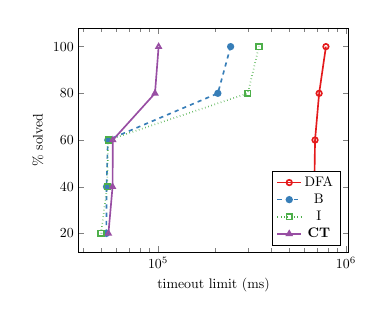
\begin{tikzpicture}[scale=0.5]
      \begin{axis}[
    xmode=log,
    every axis plot/.style={thin},
    xlabel={timeout limit (ms)},
    ylabel={\% solved},
    legend pos=south east,
    cycle list/Set1-6,
            % define fill color for the marker
            mark list fill={.!75!white},
            mark options={solid},
            cycle multiindex* list={
                Set1-6
                    \nextlist
                [3 of]linestyles
                    \nextlist
                very thick
                \nextlist
                mark=o,
                mark=*,
                mark=square,
                mark=triangle,
                mark=+
            },
    ]

    \addplot
    coordinates {
      (650070, 20)
      (678420, 40)
      (684190, 60)
      (719490, 80)
      (781960, 100)
      
    };
    \addplot
    coordinates {
      (53070, 20)
      (53180, 40)
      (54030, 60)
      (208000, 80)
      (243230, 100)
      
    };
    \addplot
    coordinates {
      (49740, 20)
      (53570, 40)
      (54260, 60)
      (300160, 80)
      (344290, 100)
      
    };
    \addplot
    coordinates {
      (54430, 20)
      (57260, 40)
      (57450, 60)
      (96290, 80)
      (100660, 100)
      
    };
    

    \legend{ DFA, B, I, \textbf{CT} }
  \end{axis}

    \end{tikzpicture}
    &
      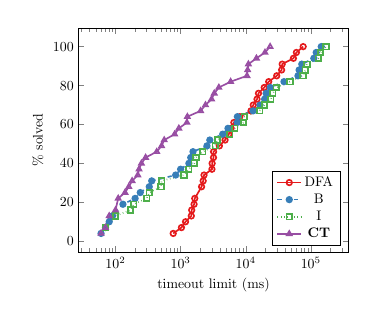
\begin{tikzpicture}[scale=0.5]
        \begin{axis}[
    xmode=log,
    every axis plot/.style={thin},
    xlabel={timeout limit (ms)},
    ylabel={\% solved},
    legend pos=south east,
    cycle list/Set1-6,
            % define fill color for the marker
            mark list fill={.!75!white},
            mark options={solid},
            cycle multiindex* list={
                Set1-6
                    \nextlist
                [3 of]linestyles
                    \nextlist
                very thick
                \nextlist
                mark=o,
                mark=*,
                mark=square,
                mark=triangle,
                mark=+
            },
    ]

    \addplot
    coordinates {
      (770, 4)
      (1030, 7)
      (1190, 10)
      (1460, 13)
      (1480, 16)
      (1610, 19)
      (1650, 22)
      (2100, 28)
      (2220, 31)
      (2290, 34)
      (3030, 37)
      (3050, 40)
      (3200, 43)
      (3210, 46)
      (3940, 49)
      (4820, 52)
      (5510, 55)
      (5960, 58)
      (6580, 61)
      (8120, 64)
      (12080, 67)
      (13060, 70)
      (14920, 73)
      (15710, 76)
      (19260, 79)
      (22550, 82)
      (29920, 85)
      (35600, 88)
      (36330, 91)
      (54060, 94)
      (60090, 97)
      (76370, 100)
      
    };
    \addplot
    coordinates {
      (60, 4)
      (70, 7)
      (80, 10)
      (90, 13)
      (130, 19)
      (200, 22)
      (240, 25)
      (330, 28)
      (360, 31)
      (840, 34)
      (1000, 37)
      (1340, 40)
      (1430, 43)
      (1550, 46)
      (2540, 49)
      (2810, 52)
      (4430, 55)
      (5340, 58)
      (7400, 61)
      (7450, 64)
      (12980, 67)
      (16570, 70)
      (19500, 73)
      (20590, 76)
      (23780, 79)
      (38770, 82)
      (63540, 85)
      (66170, 88)
      (72660, 91)
      (111260, 94)
      (121100, 97)
      (144690, 100)
      
    };
    \addplot
    coordinates {
      (70, 7)
      (100, 13)
      (170, 16)
      (190, 19)
      (300, 22)
      (330, 25)
      (500, 28)
      (510, 31)
      (1130, 34)
      (1330, 37)
      (1620, 40)
      (1720, 43)
      (2180, 46)
      (3390, 49)
      (3680, 52)
      (5660, 55)
      (6820, 58)
      (9260, 61)
      (9470, 64)
      (16340, 67)
      (19480, 70)
      (24380, 73)
      (26140, 76)
      (29480, 79)
      (47910, 82)
      (75650, 85)
      (82650, 88)
      (87290, 91)
      (130370, 94)
      (140830, 97)
      (170720, 100)
      
    };
    \addplot
    coordinates {
      (60, 4)
      (70, 7)
      (80, 13)
      (100, 16)
      (110, 22)
      (140, 25)
      (160, 28)
      (180, 31)
      (220, 34)
      (230, 37)
      (250, 40)
      (290, 43)
      (430, 46)
      (510, 49)
      (560, 52)
      (810, 55)
      (940, 58)
      (1250, 61)
      (1270, 64)
      (2030, 67)
      (2410, 70)
      (2990, 73)
      (3290, 76)
      (3870, 79)
      (5870, 82)
      (10460, 85)
      (10710, 88)
      (11000, 91)
      (14610, 94)
      (19780, 97)
      (23710, 100)
      
    };
    

    \legend{ DFA, B, I, \textbf{CT} }
  \end{axis}

      \end{tikzpicture} \\
    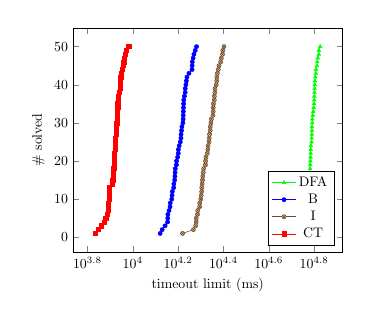
\begin{tikzpicture}[scale=0.5]
      \begin{axis}[
    xmode=log,
    every axis plot/.style={thin},
    xlabel={timeout limit (ms)},
    ylabel={\# solved},
    legend pos=south east
    % table/create on use/cumulative distribution/.style={
    %   create col/expr={\pgfmathaccuma + \thisrow{f(x)}}   
    % }
    ]
    \addplot 
    [mark=triangle*,
    mark size=1.5,
    mark options={solid},
    green] 
    coordinates {
    (51125.785, 1)
(54263.257, 2)
(56487.527, 3)
(56702.786, 4)
(56985.792, 5)
(57276.885, 6)
(57622.584, 7)
(58132.270, 8)
(58140.300, 9)
(58355.175, 10)
(58676.203, 11)
(59158.883, 12)
(59632.816, 13)
(59713.900, 14)
(59728.215, 15)
(60269.934, 16)
(60313.648, 17)
(60549.505, 18)
(60622.637, 19)
(60711.449, 20)
(60810.980, 21)
(60862.784, 22)
(60914.293, 23)
(61100.454, 24)
(61428.994, 25)
(61523.477, 26)
(61625.366, 27)
(61712.915, 28)
(61729.236, 29)
(61886.596, 30)
(61900.845, 31)
(62341.893, 32)
(62455.546, 33)
(62817.572, 34)
(63010.646, 35)
(63184.232, 36)
(63221.376, 37)
(63304.994, 38)
(63379.424, 39)
(63540.272, 40)
(63613.419, 41)
(63781.589, 42)
(64128.455, 43)
(64263.902, 44)
(64924.220, 45)
(65113.900, 46)
(65508.695, 47)
(66133.866, 48)
(66157.482, 49)
(67076.860, 50)
    };

    \addplot 
    [blue,
    mark=*,
    mark size=1.5,
    mark options={solid}]
    coordinates {
    (13210.645, 1)
(13478.699, 2)
(13880.904, 3)
(14240.906, 4)
(14262.586, 5)
(14281.012, 6)
(14453.879, 7)
(14601.257, 8)
(14630.915, 9)
(14856.229, 10)
(14906.587, 11)
(14947.426, 12)
(15147.432, 13)
(15173.599, 14)
(15300.351, 15)
(15338.350, 16)
(15370.471, 17)
(15400.162, 18)
(15575.398, 19)
(15599.555, 20)
(15767.367, 21)
(15876.487, 22)
(15890.540, 23)
(16026.936, 24)
(16207.081, 25)
(16313.213, 26)
(16328.178, 27)
(16410.911, 28)
(16468.425, 29)
(16641.910, 30)
(16678.794, 31)
(16689.212, 32)
(16716.749, 33)
(16728.322, 34)
(16755.929, 35)
(16780.814, 36)
(16896.779, 37)
(17026.619, 38)
(17037.921, 39)
(17147.387, 40)
(17237.324, 41)
(17326.549, 42)
(17685.575, 43)
(18266.956, 44)
(18281.157, 45)
(18310.293, 46)
(18466.165, 47)
(18608.783, 48)
(18864.433, 49)
(19102.683, 50)
    };

    \addplot [brown!60!black,
    mark options={fill=brown!40},
    mark=otimes*,
    mark size=1.5]
    coordinates {
    (16575.843, 1)
(18505.000, 2)
(18940.008, 3)
(19038.980, 4)
(19049.304, 5)
(19298.221, 6)
(19348.596, 7)
(19719.698, 8)
(19737.753, 9)
(19947.661, 10)
(20036.932, 11)
(20122.714, 12)
(20152.397, 13)
(20232.116, 14)
(20302.198, 15)
(20360.843, 16)
(20458.853, 17)
(20543.247, 18)
(20924.864, 19)
(20941.580, 20)
(21033.055, 21)
(21323.434, 22)
(21424.912, 23)
(21488.205, 24)
(21690.524, 25)
(21732.563, 26)
(21805.424, 27)
(21961.943, 28)
(21968.175, 29)
(22103.640, 30)
(22217.515, 31)
(22576.655, 32)
(22629.332, 33)
(22640.426, 34)
(22690.290, 35)
(22898.044, 36)
(22906.588, 37)
(23018.632, 38)
(23049.661, 39)
(23346.986, 40)
(23464.371, 41)
(23482.242, 42)
(23611.320, 43)
(23844.593, 44)
(24011.531, 45)
(24420.146, 46)
(24590.635, 47)
(24882.878, 48)
(24954.062, 49)
(25252.813, 50)
    };

    \addplot 
    [red,
    mark size=1.5,
    mark=square*]
    coordinates {
    (6834.272, 1)
(7049.566, 2)
(7238.120, 3)
(7457.754, 4)
(7598.772, 5)
(7739.737, 6)
(7771.586, 7)
(7772.970, 8)
(7812.433, 9)
(7861.439, 10)
(7862.003, 11)
(7867.552, 12)
(7871.233, 13)
(8146.006, 14)
(8162.853, 15)
(8169.022, 16)
(8197.217, 17)
(8246.900, 18)
(8258.157, 19)
(8262.374, 20)
(8291.516, 21)
(8318.251, 22)
(8342.451, 23)
(8355.561, 24)
(8389.425, 25)
(8401.690, 26)
(8470.665, 27)
(8475.034, 28)
(8489.871, 29)
(8495.761, 30)
(8507.506, 31)
(8510.152, 32)
(8560.945, 33)
(8587.622, 34)
(8588.072, 35)
(8642.789, 36)
(8662.209, 37)
(8738.285, 38)
(8798.802, 39)
(8820.422, 40)
(8831.432, 41)
(8851.771, 42)
(8928.438, 43)
(8949.293, 44)
(9107.856, 45)
(9118.812, 46)
(9135.516, 47)
(9225.896, 48)
(9370.806, 49)
(9607.234, 50)
    };
    \legend{DFA,B,I,CT}
  \end{axis}

    \end{tikzpicture}
    &
      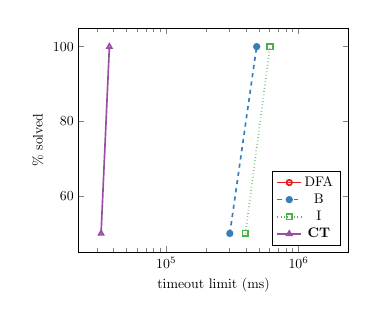
\begin{tikzpicture}[scale=0.5]
        \begin{axis}[
    xmode=log,
    every axis plot/.style={thin},
    xlabel={timeout limit (ms)},
    ylabel={\% solved},
    legend pos=south east,
    cycle list/Set1-6,
            % define fill color for the marker
            mark list fill={.!75!white},
            mark options={solid},
            cycle multiindex* list={
                Set1-6
                    \nextlist
                [3 of]linestyles
                    \nextlist
                very thick
                \nextlist
                mark=o,
                mark=*,
                mark=square,
                mark=triangle,
                mark=+
            },
    ]

    \addplot
    coordinates {
      (1609830, 50)
      
    };
    \addplot
    coordinates {
      (302190, 50)
      (482210, 100)
      
    };
    \addplot
    coordinates {
      (396530, 50)
      (608250, 100)
      
    };
    \addplot
    coordinates {
      (32160, 50)
      (37170, 100)
      
    };
    

    \legend{ DFA, B, I, \textbf{CT} }
  \end{axis}

      \end{tikzpicture} \\
  \end{tabular}
\end{frame}


\begin{frame}
  \frametitle{Small domains}
  \framesubtitle{Domain size $2$}
  \begin{tabular}{cc}
    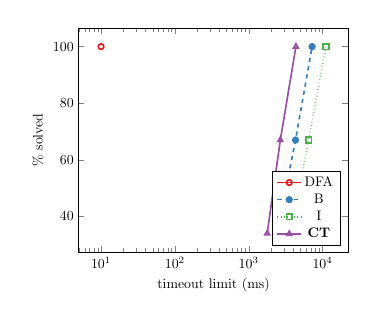
\begin{tikzpicture}[scale=0.5]
      \begin{axis}[
    xmode=log,
    every axis plot/.style={thin},
    xlabel={timeout limit (ms)},
    ylabel={\% solved},
    legend pos=south east,
    cycle list/Set1-6,
            % define fill color for the marker
            mark list fill={.!75!white},
            mark options={solid},
            cycle multiindex* list={
                Set1-6
                    \nextlist
                [3 of]linestyles
                    \nextlist
                very thick
                \nextlist
                mark=o,
                mark=*,
                mark=square,
                mark=triangle,
                mark=+
            },
    ]

    \addplot
    coordinates {
      (10, 100)
      
    };
    \addplot
    coordinates {
      (2410, 34)
      (4310, 67)
      (7220, 100)
      
    };
    \addplot
    coordinates {
      (3730, 34)
      (6480, 67)
      (11110, 100)
      
    };
    \addplot
    coordinates {
      (1780, 34)
      (2680, 67)
      (4360, 100)
      
    };
    

    \legend{ DFA, B, I, \textbf{CT} }
  \end{axis}

    \end{tikzpicture}
    &
      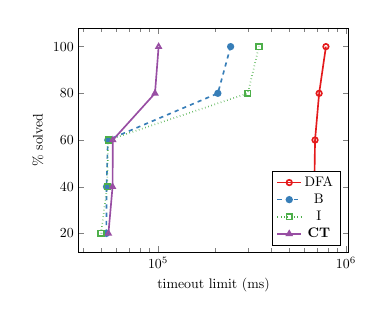
\begin{tikzpicture}[scale=0.5]
        \begin{axis}[
    xmode=log,
    every axis plot/.style={thin},
    xlabel={timeout limit (ms)},
    ylabel={\% solved},
    legend pos=south east,
    cycle list/Set1-6,
            % define fill color for the marker
            mark list fill={.!75!white},
            mark options={solid},
            cycle multiindex* list={
                Set1-6
                    \nextlist
                [3 of]linestyles
                    \nextlist
                very thick
                \nextlist
                mark=o,
                mark=*,
                mark=square,
                mark=triangle,
                mark=+
            },
    ]

    \addplot
    coordinates {
      (650070, 20)
      (678420, 40)
      (684190, 60)
      (719490, 80)
      (781960, 100)
      
    };
    \addplot
    coordinates {
      (53070, 20)
      (53180, 40)
      (54030, 60)
      (208000, 80)
      (243230, 100)
      
    };
    \addplot
    coordinates {
      (49740, 20)
      (53570, 40)
      (54260, 60)
      (300160, 80)
      (344290, 100)
      
    };
    \addplot
    coordinates {
      (54430, 20)
      (57260, 40)
      (57450, 60)
      (96290, 80)
      (100660, 100)
      
    };
    

    \legend{ DFA, B, I, \textbf{CT} }
  \end{axis}

      \end{tikzpicture} \\
    \end{tabular}
\end{frame}

\begin{frame}
  \frametitle{Large domains}
  \framesubtitle{Domain size $\geq 10$}
  \begin{tabular}{cc}
    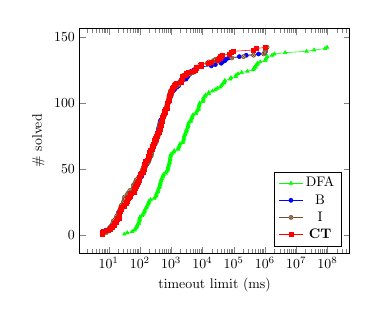
\begin{tikzpicture}[scale=0.5]
      \begin{axis}[
    xmode=log,
    every axis plot/.style={thin},
    xlabel={timeout limit (ms)},
    ylabel={\# solved},
    legend pos=south east
    % table/create on use/cumulative distribution/.style={
    %   create col/expr={\pgfmathaccuma + \thisrow{f(x)}}   
    % }
    ]
    \addplot 
    [mark=triangle*,
    mark size=1.5,
    mark options={solid},
    green] 
    coordinates {
    (31.696, 1)
(39.559, 2)
(56.508, 3)
(68.178, 4)
(70.931, 5)
(75.984, 6)
(81.689, 7)
(82.437, 8)
(90.551, 9)
(92.696, 10)
(96.318, 11)
(97.489, 12)
(98.251, 13)
(100.928, 14)
(116.739, 15)
(124.823, 16)
(132.967, 17)
(139.159, 18)
(141.636, 19)
(149.509, 20)
(161.219, 21)
(165.144, 22)
(176.745, 23)
(182.586, 24)
(193.826, 25)
(196.443, 26)
(220.596, 27)
(287.801, 28)
(307.637, 29)
(331.351, 30)
(335.110, 31)
(344.194, 32)
(377.529, 33)
(378.932, 34)
(389.655, 35)
(410.350, 36)
(423.248, 37)
(438.655, 38)
(450.859, 39)
(454.186, 40)
(475.260, 41)
(483.019, 42)
(493.122, 43)
(544.266, 44)
(544.377, 45)
(568.390, 46)
(658.959, 47)
(704.627, 48)
(733.115, 49)
(790.697, 50)
(796.819, 51)
(799.668, 52)
(839.106, 53)
(863.117, 54)
(884.469, 55)
(886.545, 56)
(921.009, 57)
(927.374, 58)
(928.500, 59)
(970.121, 60)
(970.451, 61)
(1084.311, 62)
(1214.035, 63)
(1256.732, 64)
(1667.050, 65)
(1679.067, 66)
(1790.603, 67)
(1813.082, 68)
(1923.256, 69)
(2334.693, 70)
(2424.581, 71)
(2460.778, 72)
(2524.488, 73)
(2535.289, 74)
(2608.483, 75)
(2727.527, 76)
(2790.777, 77)
(3010.831, 78)
(3089.396, 79)
(3100.186, 80)
(3342.097, 81)
(3421.319, 82)
(3476.286, 83)
(3498.766, 84)
(3603.983, 85)
(4152.208, 86)
(4252.733, 87)
(4414.005, 88)
(4619.485, 89)
(4703.303, 90)
(4995.143, 91)
(6104.482, 92)
(6327.657, 93)
(6680.221, 94)
(7451.205, 95)
(7524.283, 96)
(7577.742, 97)
(7815.366, 98)
(7963.806, 99)
(8190.616, 100)
(10239.338, 101)
(10646.387, 102)
(10743.772, 103)
(10816.354, 104)
(12183.647, 105)
(12608.953, 106)
(15986.466, 107)
(16016.047, 108)
(21085.457, 109)
(25840.612, 110)
(30330.074, 111)
(37303.992, 112)
(39784.632, 113)
(42867.757, 114)
(49654.939, 115)
(49896.816, 116)
(51937.811, 117)
(76626.715, 118)
(81762.693, 119)
(116690.715, 120)
(118979.114, 121)
(138352.575, 122)
(179596.690, 123)
(275896.959, 124)
(422494.853, 125)
(435710.733, 126)
(490650.459, 127)
(500154.998, 128)
(546044.177, 129)
(592457.334, 130)
(707795.890, 131)
(1014847.682, 132)
(1051973.108, 133)
(1109712.990, 134)
(1188811.633, 135)
(1691073.549, 136)
(1998815.209, 137)
(4412151.304, 138)
(21464315.090, 139)
(37446981.305, 140)
(83163795.720, 141)
(97236200.525, 142)
    };

    \addplot 
    [blue,
    mark=*,
    mark size=1.5,
    mark options={solid}]
    coordinates {
    (6.266, 1)
(6.620, 2)
(7.191, 3)
(8.174, 4)
(10.291, 5)
(11.099, 6)
(12.126, 7)
(13.714, 8)
(14.201, 9)
(17.122, 10)
(17.173, 11)
(18.736, 12)
(19.358, 13)
(19.989, 14)
(20.187, 15)
(20.291, 16)
(20.437, 17)
(21.788, 18)
(22.787, 19)
(26.326, 20)
(28.086, 21)
(28.501, 22)
(30.269, 23)
(30.327, 24)
(31.429, 25)
(32.957, 26)
(35.312, 27)
(37.683, 28)
(42.027, 29)
(44.010, 30)
(45.270, 31)
(57.413, 32)
(58.136, 33)
(60.287, 34)
(63.612, 35)
(64.377, 36)
(70.203, 37)
(71.636, 38)
(74.510, 39)
(81.417, 40)
(81.885, 41)
(86.850, 42)
(98.379, 43)
(110.554, 44)
(114.955, 45)
(116.342, 46)
(116.797, 47)
(117.697, 48)
(127.569, 49)
(128.638, 50)
(132.319, 51)
(149.619, 52)
(156.554, 53)
(167.748, 54)
(171.866, 55)
(177.579, 56)
(186.974, 57)
(188.731, 58)
(197.746, 59)
(206.427, 60)
(212.854, 61)
(223.093, 62)
(234.349, 63)
(237.887, 64)
(249.281, 65)
(261.335, 66)
(279.625, 67)
(282.633, 68)
(287.627, 69)
(297.860, 70)
(315.101, 71)
(322.909, 72)
(331.748, 73)
(351.193, 74)
(352.948, 75)
(363.872, 76)
(366.739, 77)
(390.571, 78)
(395.284, 79)
(397.359, 80)
(399.002, 81)
(410.756, 82)
(418.082, 83)
(436.759, 84)
(439.198, 85)
(447.297, 86)
(462.840, 87)
(504.442, 88)
(543.477, 89)
(559.175, 90)
(566.240, 91)
(601.149, 92)
(619.715, 93)
(652.612, 94)
(657.839, 95)
(715.983, 96)
(731.157, 97)
(752.783, 98)
(784.906, 99)
(794.121, 100)
(856.340, 101)
(862.438, 102)
(901.933, 103)
(927.762, 104)
(979.127, 105)
(1000.759, 106)
(1023.428, 107)
(1067.513, 108)
(1074.968, 109)
(1265.279, 110)
(1331.799, 111)
(1538.059, 112)
(1731.374, 113)
(1737.023, 114)
(1790.519, 115)
(1895.419, 116)
(2041.525, 117)
(2975.267, 118)
(3105.441, 119)
(3430.058, 120)
(3574.657, 121)
(3985.434, 122)
(4137.262, 123)
(4364.834, 124)
(5314.336, 125)
(6189.835, 126)
(6463.719, 127)
(19294.688, 128)
(25874.502, 129)
(40075.340, 130)
(44076.314, 131)
(52831.470, 132)
(56117.125, 133)
(69049.283, 134)
(151946.681, 135)
(251788.612, 136)
(624723.233, 137)
(1006224.760, 138)
(1024927.746, 139)
(1025126.900, 140)
(1051096.785, 141)
(1054709.554, 142)
    };

    \addplot [brown!60!black,
    mark options={fill=brown!40},
    mark=otimes*,
    mark size=1.5]
    coordinates {
    (6.225, 1)
(8.252, 2)
(8.866, 3)
(8.903, 4)
(10.276, 5)
(10.793, 6)
(12.246, 7)
(12.967, 8)
(13.482, 9)
(13.873, 10)
(14.125, 11)
(15.975, 12)
(17.388, 13)
(17.590, 14)
(18.641, 15)
(20.043, 16)
(20.476, 17)
(21.613, 18)
(23.615, 19)
(24.164, 20)
(24.372, 21)
(24.882, 22)
(26.053, 23)
(29.400, 24)
(29.513, 25)
(30.549, 26)
(31.898, 27)
(32.205, 28)
(32.366, 29)
(39.353, 30)
(39.524, 31)
(42.127, 32)
(45.853, 33)
(48.185, 34)
(60.297, 35)
(60.940, 36)
(61.286, 37)
(61.970, 38)
(67.684, 39)
(71.354, 40)
(74.374, 41)
(76.755, 42)
(86.492, 43)
(92.532, 44)
(102.074, 45)
(107.118, 46)
(110.458, 47)
(119.452, 48)
(120.692, 49)
(122.537, 50)
(130.211, 51)
(131.757, 52)
(139.069, 53)
(139.341, 54)
(184.184, 55)
(187.471, 56)
(198.576, 57)
(201.040, 58)
(207.945, 59)
(229.958, 60)
(232.188, 61)
(233.976, 62)
(239.163, 63)
(240.688, 64)
(241.932, 65)
(243.311, 66)
(245.547, 67)
(265.954, 68)
(292.029, 69)
(328.546, 70)
(334.072, 71)
(336.358, 72)
(350.752, 73)
(375.324, 74)
(379.234, 75)
(396.967, 76)
(401.683, 77)
(401.895, 78)
(405.570, 79)
(411.227, 80)
(417.570, 81)
(419.966, 82)
(421.977, 83)
(456.664, 84)
(458.121, 85)
(467.458, 86)
(514.809, 87)
(537.183, 88)
(573.529, 89)
(585.083, 90)
(628.983, 91)
(629.151, 92)
(638.579, 93)
(655.494, 94)
(683.596, 95)
(719.854, 96)
(720.103, 97)
(726.177, 98)
(743.018, 99)
(776.859, 100)
(788.068, 101)
(801.667, 102)
(840.869, 103)
(844.819, 104)
(845.660, 105)
(882.665, 106)
(896.694, 107)
(936.968, 108)
(941.257, 109)
(1025.243, 110)
(1127.272, 111)
(1290.616, 112)
(1527.467, 113)
(1798.817, 114)
(1803.072, 115)
(1966.245, 116)
(2089.371, 117)
(2225.216, 118)
(2378.815, 119)
(2497.087, 120)
(2503.823, 121)
(3943.794, 122)
(5004.718, 123)
(5143.946, 124)
(5663.752, 125)
(6369.410, 126)
(6913.053, 127)
(8260.886, 128)
(8382.946, 129)
(14367.240, 130)
(16013.595, 131)
(22433.224, 132)
(26100.534, 133)
(86936.175, 134)
(206857.036, 135)
(432302.057, 136)
(923791.300, 137)
(1001275.049, 138)
(1005552.392, 139)
(1024252.398, 140)
(1082346.127, 141)
(1174868.682, 142)
    };

    \addplot 
    [red,
    mark size=1.5,
    mark=square*]
    coordinates {
    (6.328, 1)
(6.344, 2)
(6.785, 3)
(9.703, 4)
(11.389, 5)
(12.785, 6)
(13.199, 7)
(14.710, 8)
(15.330, 9)
(17.053, 10)
(17.466, 11)
(18.730, 12)
(21.191, 13)
(21.458, 14)
(22.190, 15)
(22.321, 16)
(22.429, 17)
(23.230, 18)
(23.566, 19)
(24.810, 20)
(24.843, 21)
(30.529, 22)
(31.162, 23)
(35.615, 24)
(37.410, 25)
(38.475, 26)
(38.831, 27)
(43.209, 28)
(45.793, 29)
(47.775, 30)
(48.066, 31)
(53.755, 32)
(65.633, 33)
(66.267, 34)
(66.798, 35)
(69.198, 36)
(73.621, 37)
(77.636, 38)
(83.309, 39)
(87.127, 40)
(87.800, 41)
(92.901, 42)
(93.082, 43)
(98.471, 44)
(101.548, 45)
(102.853, 46)
(112.950, 47)
(126.755, 48)
(126.916, 49)
(133.777, 50)
(136.483, 51)
(139.301, 52)
(141.708, 53)
(142.901, 54)
(147.720, 55)
(151.267, 56)
(167.047, 57)
(180.053, 58)
(185.002, 59)
(192.458, 60)
(199.346, 61)
(200.444, 62)
(205.194, 63)
(211.032, 64)
(245.046, 65)
(247.635, 66)
(258.985, 67)
(273.140, 68)
(274.226, 69)
(289.992, 70)
(293.258, 71)
(296.666, 72)
(320.259, 73)
(325.794, 74)
(331.950, 75)
(359.459, 76)
(369.740, 77)
(401.942, 78)
(428.598, 79)
(439.186, 80)
(443.919, 81)
(451.155, 82)
(465.721, 83)
(486.636, 84)
(496.533, 85)
(507.498, 86)
(509.344, 87)
(518.391, 88)
(534.298, 89)
(549.969, 90)
(554.731, 91)
(594.595, 92)
(623.445, 93)
(624.194, 94)
(658.888, 95)
(748.721, 96)
(754.742, 97)
(754.776, 98)
(757.089, 99)
(766.244, 100)
(789.618, 101)
(856.352, 102)
(878.697, 103)
(882.688, 104)
(885.633, 105)
(948.909, 106)
(961.811, 107)
(1025.381, 108)
(1027.979, 109)
(1068.881, 110)
(1096.069, 111)
(1141.179, 112)
(1263.836, 113)
(1363.480, 114)
(1444.963, 115)
(2086.545, 116)
(2104.289, 117)
(2266.072, 118)
(2315.715, 119)
(2337.155, 120)
(2809.498, 121)
(3062.328, 122)
(3613.655, 123)
(4962.131, 124)
(5757.448, 125)
(6278.281, 126)
(6458.606, 127)
(9074.926, 128)
(9388.538, 129)
(15237.846, 130)
(19012.640, 131)
(29844.102, 132)
(32057.652, 133)
(36009.393, 134)
(38516.958, 135)
(44360.448, 136)
(70712.723, 137)
(84815.013, 138)
(99208.278, 139)
(426595.818, 140)
(513749.533, 141)
(1012388.065, 142)
    };
    \legend{DFA,B,I,\textbf{CT}}
  \end{axis}

    \end{tikzpicture}
    &
      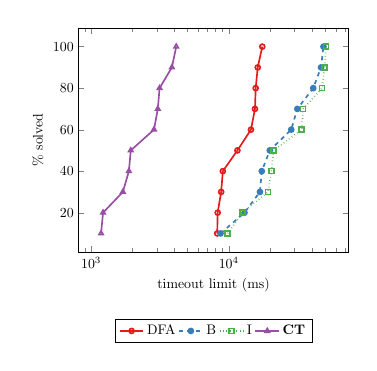
\begin{tikzpicture}[scale=0.5]
        \begin{axis}[
    xmode=log,
    every axis plot/.style={thin},
    xlabel={timeout limit (ms)},
    ylabel={\% solved},
    legend style={at={(0.5,-0.30)},
      anchor=north,legend columns=-1},
    % legend pos=south east,
    cycle list/Set1-6,
            % define fill color for the marker
            mark list fill={.!75!white},
            mark options={solid,scale=0.9},
            cycle multiindex* list={
                Set1-6
                    \nextlist
                [3 of]linestyles
                    \nextlist
                very thick
                \nextlist
                mark=o,
                mark=*,
                mark=square,
                mark=triangle,
                mark=+
            },
    ]

    \addplot
    coordinates {
      (8240, 10)
      (8300, 20)
      (8800, 30)
      (9050, 40)
      (11550, 50)
      (14490, 60)
      (15490, 70)
      (15680, 80)
      (16230, 90)
      (17510, 100)
      
    };
    \addplot
    coordinates {
      (8710, 10)
      (13000, 20)
      (16840, 30)
      (17370, 40)
      (19860, 50)
      (28430, 60)
      (31470, 70)
      (41080, 80)
      (46790, 90)
      (48720, 100)
      
    };
    \addplot
    coordinates {
      (9810, 10)
      (12550, 20)
      (19300, 30)
      (20370, 40)
      (21220, 50)
      (33870, 60)
      (34700, 70)
      (47590, 80)
      (49800, 90)
      (50780, 100)
      
    };
    \addplot
    coordinates {
      (1180, 10)
      (1220, 20)
      (1700, 30)
      (1880, 40)
      (1940, 50)
      (2860, 60)
      (3050, 70)
      (3140, 80)
      (3860, 90)
      (4150, 100)
      
    };
    

    \legend{ DFA, B, I, \textbf{CT} }
  \end{axis}

      \end{tikzpicture} \\
  \end{tabular}
\end{frame}

\begin{frame}
  \frametitle{Results}
  \begin{itemize}
    \item CT seems to outperfom the other propagators
    \item CT has largest performance gains on series with large tables
    \item DFA overall slowest
  \end{itemize}
\end{frame}

\section{Summary and Conclusions}

\begin{frame}
  \frametitle{Summary and Conclusions}
  \begin{itemize}
  \item   What I have done:
    \begin{itemize}
    \item Implemented Compact-Table (CT) in Gecode
    \item Compared CT against existing propagators for \Table,
      and with \Constraint{Regular}
    \end{itemize}
  \item   The results:
    \begin{itemize}
      \item CT seems to outperform existing propagators for \Table
    \end{itemize}
    % \item Remains to be done:
    %   \begin{itemize}
    %     \item Find a bug
    %   \end{itemize}
    \item Future work:
      \begin{itemize}
      \item Proof of concept -- not a final version
      \item Inclusion into Gecode?
      \item Implement and evaluate generalisations of CT described
        in~\cite{DBLP:conf/aaai/VerhaegheLS17}
      \end{itemize}
  
  \end{itemize}
\end{frame}

\begin{frame}
  \frametitle{References}
  \printbibliography
  %\begin{thebibliography}{9}
    
  %\bibitem[Demeulenaere, Hartert, Lecoutre, Perez, Perron, R{\'{e}}gin, and Schaus @ CP 2016]{CTpaper} Demeulenaere, J. and Hartert, R. and Lecoutre, C. and Perez, G. and Perron, L. and R{\'{e}}gin, J.C. and Schaus, P.
%   \bibitem[1]{CTpaper} Demeulenaere, J. and Hartert, R. and Lecoutre, C. and Perez, G. and Perron, L. and R{\'{e}}gin, J.C. and Schaus, P.
%     \newblock Compact-Table: Efficiently Filtering Table Constraints with Reversible
%     Sparse Bit-Sets
%     \newblock \emph{Proceedings of CP 2016}, Lecture Notes in Computer Science 9892, pages 207--223. Springer, 2016.
    

% %  \bibitem[Verhaeghe, Lecoutre, and Schaus @ AAAI 2017]{CTpaper2} Verhaeghe, H{\'{e}}l{\`{e}}ne and Lecoutre, Christophe and Schaus, Pierre
%   \bibitem[2]{CTpaper2} Verhaeghe, H{\'{e}}l{\`{e}}ne and Lecoutre, Christophe and Schaus, Pierre
%     \newblock Extending Compact-Table to Negative and Short Tables,
%     \emph{Proceedings of AAAI 2017}, AAAI 2017, pages 3951--3957. AAAI Press, 2017.
               
  %\end{thebibliography}

\end{frame}

\end{document}
